\documentclass{beamer}
\usepackage[utf8]{inputenc}
\usepackage{amsmath}
\usepackage{amsfonts}
\usepackage{amssymb}
\usepackage{graphicx}
\usepackage{ragged2e}  % `\justifying` text
\usepackage{booktabs}  % Tables
\usepackage{tabularx}
\usepackage{tikz}      % Diagrams
\usetikzlibrary{calc, shapes, backgrounds}
\usepackage{amsmath}
\usepackage{amssymb}
\usepackage{dsfont}
\usepackage{url}       % `\url
\usepackage{listings}  % Code listings
\usepackage[T1]{fontenc}


\usepackage{theme/beamerthemehbrs}

\author[Ethan Oswald Massey]{Ethan Oswald Massey}
\title{Estimating Confidence in Spatio-Temporal Models}
\institute[HBRS]{Hochschule Bonn-Rhein-Sieg}
\date{2020-00-00}
%\subject{Test beamer}

\thirdpartylogo{images/ropod.png}


\begin{document}
{
\begin{frame}
\titlepage
\vspace{5mm}

Supervisiors: \\ Prof. Dr. Erwin Prassler  \\ Prof. Dr. Paul G. Pl\"{o}ger \\ M. Sc. Argentina Ortega S\'{a}inz
\end{frame}
}

\begin{frame}[t]{Uses of Spatio-Temporal Models}
  \begin{itemize}
    \setlength\itemsep{1em}
    \item Describes how an environment changes with respect to time
    \item Most useful when changes are periodic or modelable
    \item Human occupied environments are often suitable
    \item Enable improved planning, navigation, and scheduling for ROPOD
  \end{itemize}

  \begin{block}{Desired Predictions}
    \begin{itemize}
    \item Travel Time
      \begin{itemize}
        \item Elevators
        \item Hallways
      \end{itemize}
    \item Dynamic Obstacles
    \end{itemize}
  \end{block}
\end{frame}



\begin{frame}[t]{Previous Work}

  \begin{itemize}
    \item \textbf{Basic discussion about space and time complexity}
      \begin{itemize}
        \item \scriptsize FreMEn: Frequency Map Enhancement for Long-Term Mobile Robot Autonomy in Changing Environments \cite{Krajnik2015} \normalsize
        \item Comparison with Gaussian Mixture Models
      \end{itemize}


    \item \textbf{Internal comparison based on prediction accuracy}
      \begin{itemize}
        \item \scriptsize Occupancy Grid Models for Robot Mapping in Changing Environments \cite{Meyer-Delius2012} \normalsize
      \end{itemize}

    \item \textbf{Discussion of prediction accuracy and representation}
      \begin{itemize}
        \item \scriptsize A Poisson-Spectral Model for Modelling Temporal Patterns in Human Data Observed by a Robot \cite{Jovan2016} \normalsize
      \end{itemize}
  \end{itemize}

  \begin{block}{Limitations}
    \begin{itemize}
      \item Little to no comparison with other existing methods
      \item Limited in scope and depth
    \end{itemize}
  \end{block}

\end{frame}



\begin{frame}[t]{Methodology}
  \framesubtitle{What \emph{is} Confidence?}

  \begin{itemize}
    %\setlength\itemsep{1em}
    \item “The feeling or belief that one can have faith in or rely on someone or something.” \cite{Confidence2019}
    \item Epistemic vs Aleatoric uncertainty
    \item Inherent vs Introduced
    \item Predicated on data quantity and quality
  \end{itemize}

  \begin{block}{Key Concepts for this Work}
    \begin{itemize}
      \item Confidence $\simeq$ Uncertainty \cite{Geifman2018}
      \item Relies on historical knowledge/experience
      \item Driven by knowledge of spatio-temporal implementation
    \end{itemize}
  \end{block}

\end{frame}



\begin{frame}[t]{Methodology}
  \framesubtitle{Conceptual Approach to Confidence Estimation Models}
  \begin{itemize}
    \setlength\itemsep{1em}
  \item \textbf{Black Box}
      \begin{itemize}
        \item No assumptions possible
        \item Wide-reaching application
        \item Simplistic approach and results
      \end{itemize}

    \item \textbf{Grey Box}
      \begin{itemize}
        \item Some implementation knowledge needed
        \item Wide range of possible designs
        \item May require tuning
      \end{itemize}

    \item \textbf{White Box}
      \begin{itemize}
        \item Internal access and comprehension required
        \item Extremely specific
        \item Possibility for most precise and accurate results
      \end{itemize}

  \end{itemize}
\end{frame}



\begin{frame}[t]{Implementation Details}
  \framesubtitle{Use Case - ROPOD}
  \begin{columns}[t]

    \column{.5\textwidth}
    \begin{block}{What is ROPOD?}
      \begin{itemize}
        \item Autonomous multi-robot system
        \item Transports hospital beds \& supplies
        \item Deployment in human-shared environments
      \end{itemize}
    \end{block}

    \column{.5\textwidth}
    \begin{block}{Why ROPOD?}
      \begin{itemize}
        \item Real-world context
        \item Extensive opportunity for data collection
        \item Environmental representation
        \item Potential synergy with temporal planning
      \end{itemize}
    \end{block}
  \end{columns}
\end{frame}



\begin{frame}[t]{Implementation Details}
  \framesubtitle{Spatio-Temporal Model - Hypertime \cite{Krajnik2018}}
  \begin{columns}[t]

    \column{.5\textwidth}
    \begin{block}{What is Hypertime?}
      \begin{itemize}
        \item Extension of FreMEn \cite{Krajnik2015}
        \item Predicts environmental behavior or changes
        \item Binary predictions with probability
        \item Non-binary predictions with no probability
      \end{itemize}
    \end{block}

    \column{.5\textwidth}
    \begin{block}{Why Hypertime?}
      \begin{itemize}
        \item Excellent fit for ROPOD \cite{Massey2019}
        \item Fully accessible and comprehensible
        \item Lacks confidence estimates
      \end{itemize}
    \end{block}
  \end{columns}
\end{frame}



\begin{frame}[t]{Implementation Details}
  \framesubtitle{Hypertime Background and Modification}
    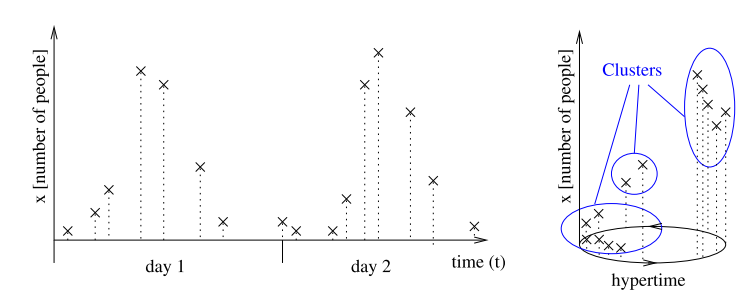
\includegraphics[width=0.80\columnwidth]{images/hypertime_clustering.png}

    \begin{block}{Hypertime Overview}
      \begin{itemize}
        \item Multiple cluster - Gaussian distributions
        \item Frequency-based representation and \& dimensionality expansion
        \item Multiple methods for predictions
      \end{itemize}
    \end{block}
\end{frame}




\begin{frame}[t]{Confidence Estimation Models}
  \framesubtitle{Data Grouping}
  \begin{itemize}
    \setlength\itemsep{1em}
  \item \textbf{Black Box - Generic Grouping}
      \begin{itemize}
        \item No assumptions possible
        \item One general grouping
      \end{itemize}

    \item \textbf{Grey Box - Temporal Groupings}
      \begin{itemize}
        \item Leverage knowledge of maximum temporal periods
        \item Divide each day of the week into three sections
      \end{itemize}

    \item \textbf{White Box - Hypertime Clusters}
      \begin{itemize}
        \item Full access and ability to modify Hypertime
        \item Modify Hypertime to indicate which cluster was used
      \end{itemize}

    \item \textbf{White X Grey Box - Combinatorial Model}
      \begin{itemize}
        \item Limited number of clusters
        \item More specific groupings may lead to more precise predictions
      \end{itemize}

  \end{itemize}
\end{frame}




\begin{frame}[t]{Confidence Estimation Models}
  \framesubtitle{Bounds Through Error Modeling }
  \begin{itemize}

      \setlength\itemsep{1em}
      \item Bounds provided by analyzing the model error during training
      \item Error is the distance from observed to predicted
      \item Divided into over and under predictions
      \item Further divided according to data grouping techniques
      \item Groups of error are analyzed to provide bounds

  \end{itemize}
\end{frame}




\begin{frame}[t]{Confidence Estimation Models}
  \framesubtitle{Bounding Techniques}
  \begin{itemize}

  %\setlength\itemsep{1em}
  \item \textbf{Variant of Confidence Interval - CI}
      \begin{itemize}
        \item Often used to address uncertainty
        \item Used in previous works \cite{Shrestha2006}
        \item Gives a range to an unknown value
        \item Bound size driven by number of observations
      \end{itemize}

    \begin{equation}
      \mu_{err} = \bar{x} + Z \frac{\sigma}{\sqrt{n}}
    \end{equation}

    \item \textbf{Two Sigma - 2$\sigma$}
      \begin{itemize}
        \item Application of the errors variance
        \item Captures a wider range of behaviors
      \end{itemize}

    \begin{equation}
      \mu_{err} = \bar{x} + 2\sigma
    \end{equation}


  \end{itemize}
\end{frame}


\begin{frame}[t]{Experimental Overview}
  \begin{itemize}
  \setlength\itemsep{1.5em}
    \item Four experiments
    \begin{enumerate}
      \item Hypertime Parameter Selection
      \item Elevator Dataset
      \item H-BRS Hallway Dataset
      \item Multi-Model Fusion Proof-of-Concept
    \end{enumerate}

    \item Five Metrics
    \begin{enumerate}
      \item Accuracy of Confidence Predictions
      \item Number of Invalid Predictions
      \item Size of Bounds
      \item Magnitude of Inaccuracy
      \item RMSE for Correct Predictions
    \end{enumerate}
  \end{itemize}
\end{frame}



\begin{frame}[t]{Elevator Dataset}
  %{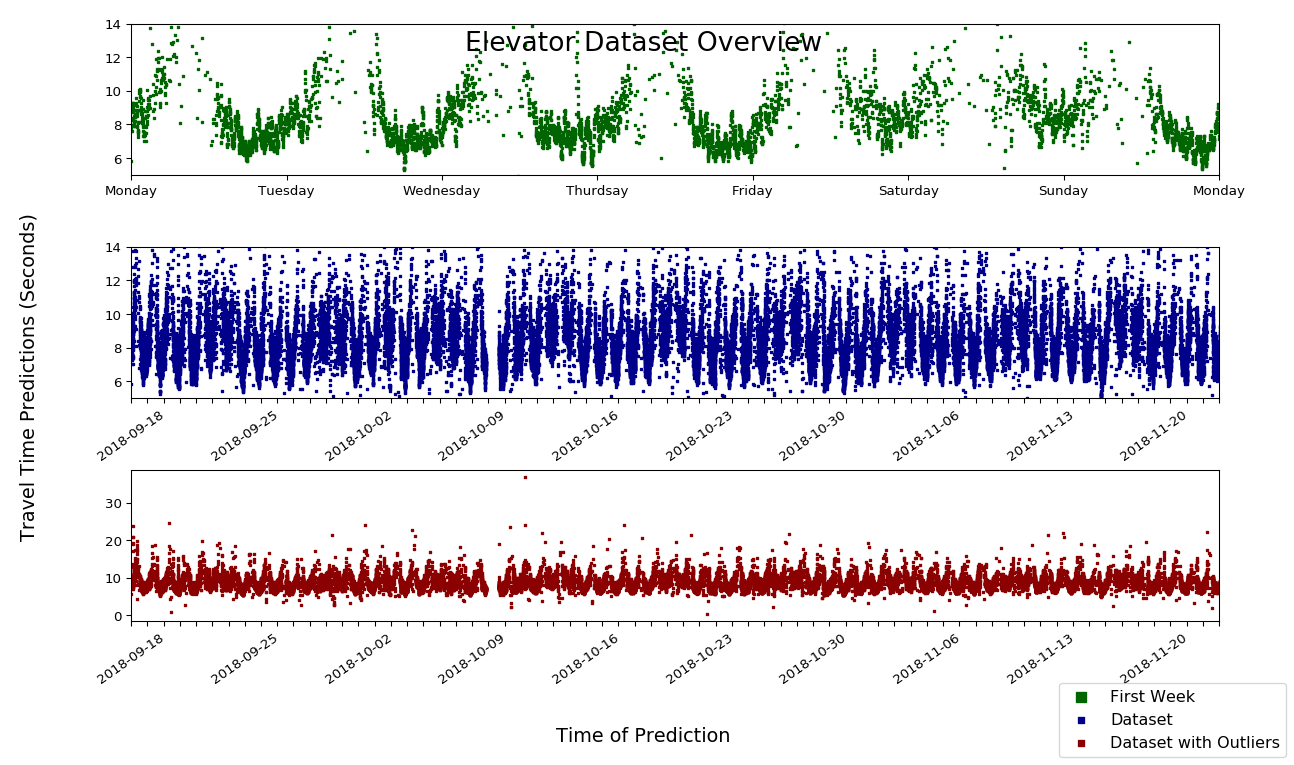
\includegraphics[width = 3.6in]{images/data_overview/elevator_dataset_overview.png}}
  \vspace*{0.40cm}
  {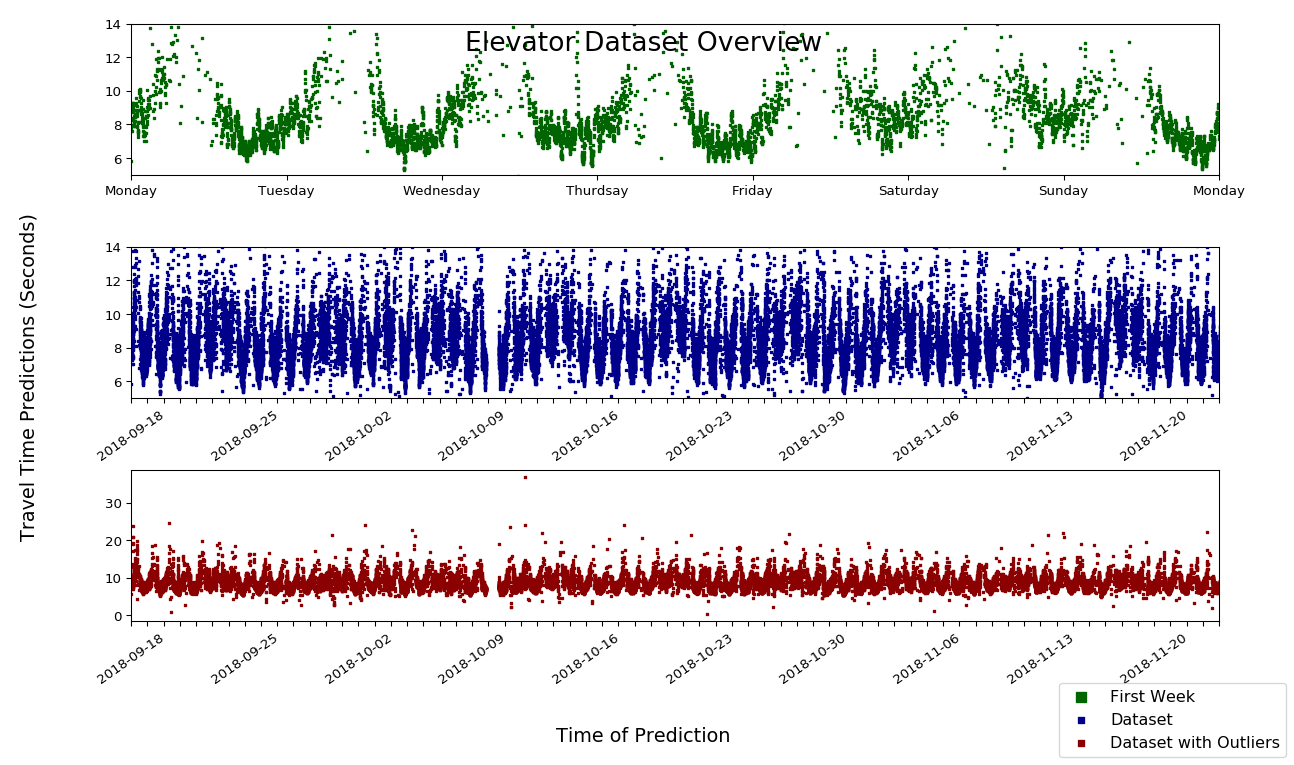
\includegraphics[width = 4.5in]{images/data_overview/elevator_dataset_overview.png}}
   % \vspace*{-0.45cm}

  %\begin{block}{Key Properties}
  %  \begin{itemize}
  %    \item Perfect Knowledge
  %    \item High Volume
  %    \item Low Noise
  %  \end{itemize}
  %\end{block}

\end{frame}



\begin{frame}[t]{Hypertime Parameter Selection}
  \framesubtitle{Determining the Optimal Parameters}
  \begin{itemize}
    %\item Determine optimal Hypertime parameters
    %\begin{enumerate}
    %  \item Number of Clusters
    %  \item Clustering Method
    %  \item Maximum Period
    %\end{enumerate}
    \setlength\itemsep{1em}

  \item \textbf{Number of Clusters}
    \begin{itemize}
      \item 1-5
    \end{itemize}
  \item \textbf{Clustering Method}
    \begin{itemize}
      \item Mean
      \item Sample Mean
      \item Sample Mode
    \end{itemize}
  \item \textbf{Maximum Period}
    \begin{itemize}
      \item One Day
      \item One Week
    \end{itemize}
  \end{itemize}
\end{frame}



\begin{frame}[t]{Hypertime Parameter Selection}

  \begin{columns}[t]
    \column{.5\textwidth}
    {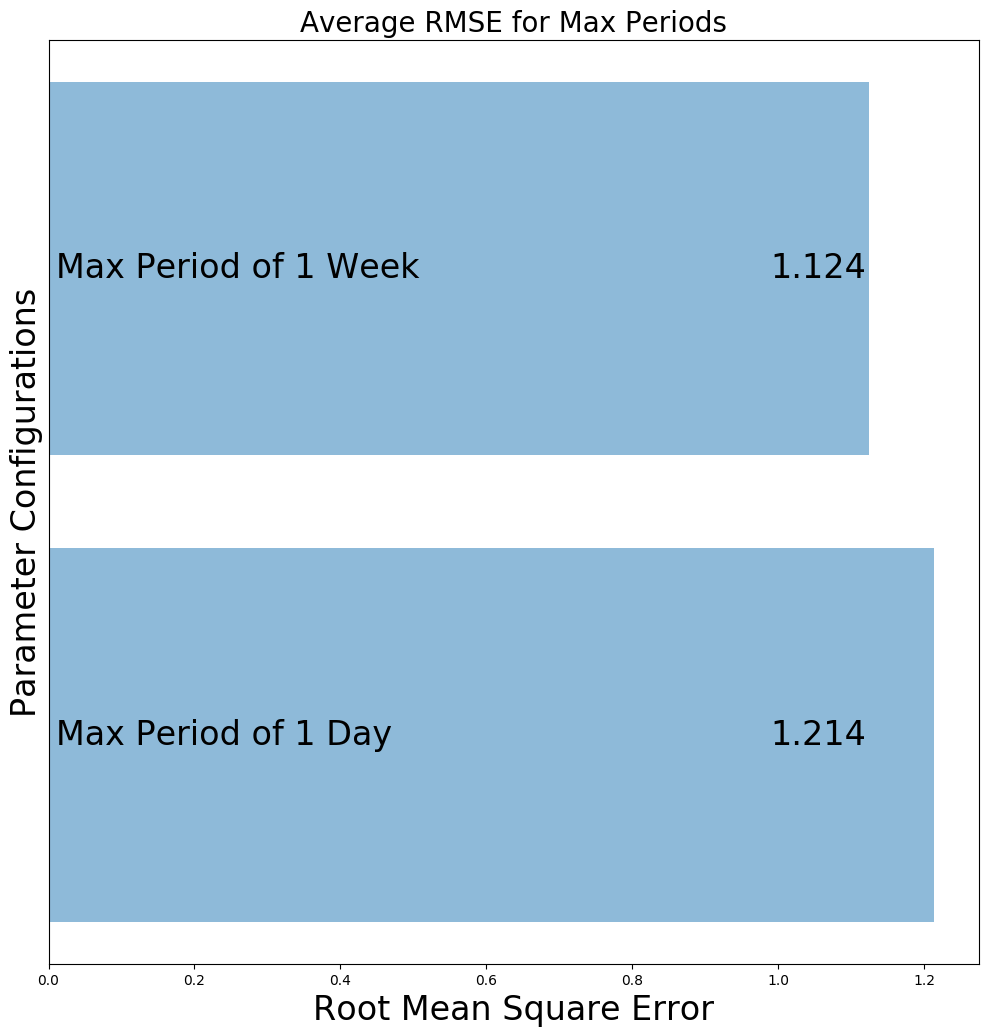
\includegraphics[width=2.3in]{images/Average_RMSE_for_Max_Periods.png}}

    \column{.5\textwidth}
    {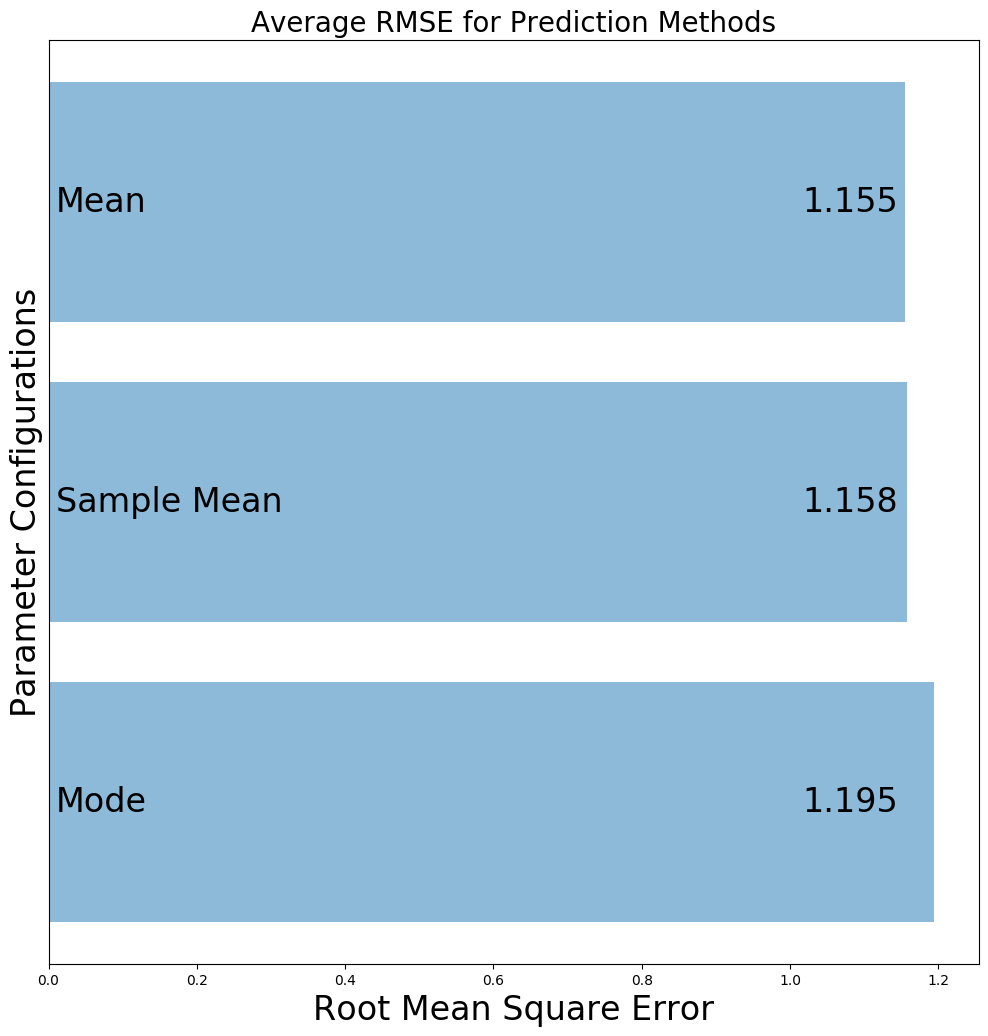
\includegraphics[width=2.3in]{images/Average_RMSE_for_Prediction_Methods.png}}
  \end{columns}

\end{frame}



\begin{frame}[t]{Hypertime Parameter Selection}
    {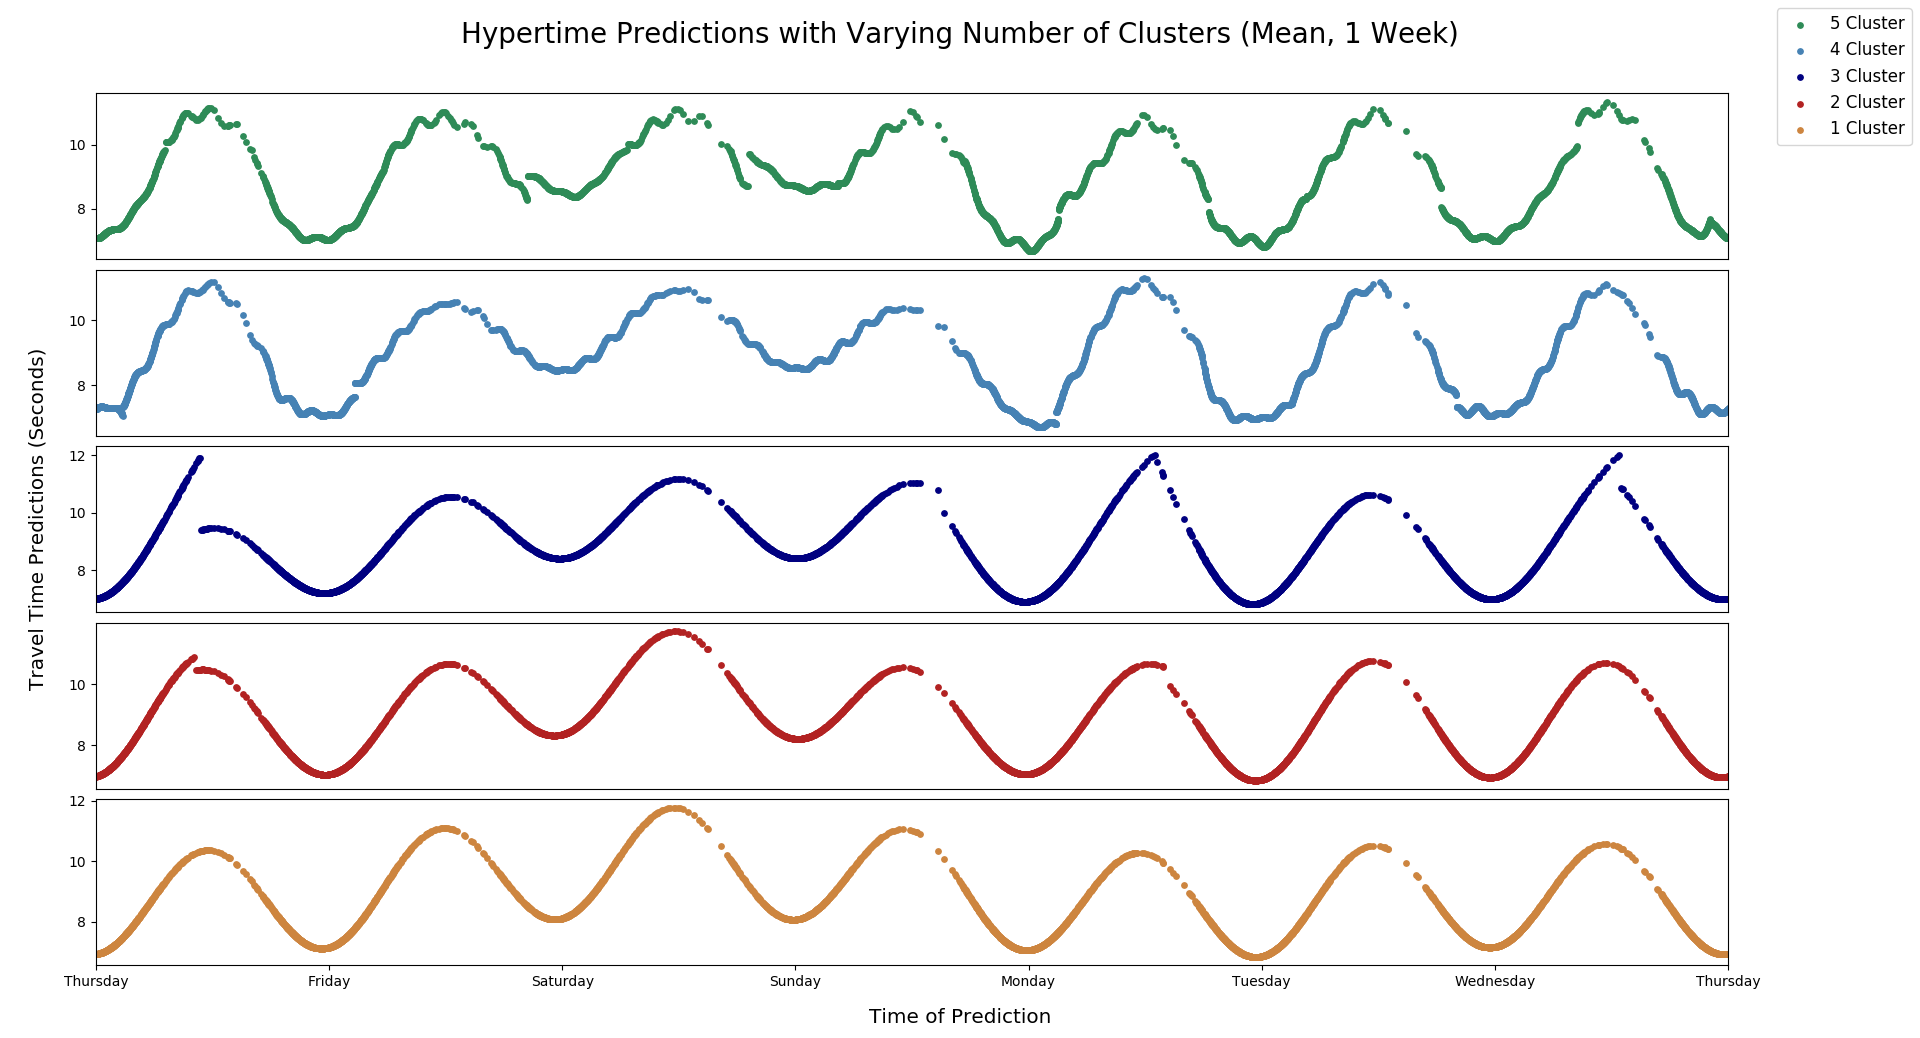
\includegraphics[width = 3.6in]{images/varying_clusters.png}}
    \vspace*{-0.45cm}

  \begin{block}{Selected Parameters}
    \begin{itemize}
      \item Number of Clusters - \textbf{5}
      \item Clustering Method - \textbf{Mean}
      \item Maximum Period - \textbf{One Week}
    \end{itemize}
  \end{block}

\end{frame}



\begin{frame}[t]{Elevator Dataset}
  \framesubtitle{Performance Under Optimal Conditions}
  \begin{itemize}
    %\item Determine optimal Hypertime parameters
    %\begin{enumerate}
    %  \item Number of Clusters
    %  \item Clustering Method
    %  \item Maximum Period
    %\end{enumerate}
    \setlength\itemsep{1em}

  \item \textbf{Effects of Data Grouping}
    \begin{itemize}
      \item Black Box
      \item Grey Box
      \item White Box
      \item White X Grey Box
    \end{itemize}
  \item \textbf{Effects of Bounding}
    \begin{itemize}
      \item Confidence Interal
      \item Two Sigma
    \end{itemize}
  \item \textbf{Effects of Sparcity}
  \end{itemize}
\end{frame}



\begin{frame}[t]{Complete Elevator Dataset}
  \framesubtitle{Overall Results}

  \vspace*{-0.5cm}
  \begin{table}[htp!]
  \small
  \begin{tabular}{|p{2.5cm}|p{1.3cm}|p{1.0cm}|p{1.7cm}|p{1.0cm}|p{1.5cm}|}

      \hline
      \textbf{Model} &
      \textbf{\% Corr.} &
      \textbf{RMSE Corr.} &
      \textbf{Magnitue of Inac.} &
      \textbf{Avg. Bound} &
      \textbf{\% Invalid} \\
      \hline

      2$\sigma$ Black Box &
      96.81\% &
      0.839 &
      0.350 &
      5.077 &
      0.00\% \\
      \hline

      2$\sigma$ Grey Box &
      96.14\% &
      0.878 &
      0.283 &
      4.562 &
      0.00\% \\
      \hline

      2$\sigma$ White Box &
      95.88\% &
      0.885 &
      0.265 &
      4.426 &
      0.00\% \\
      \hline

      2$\sigma$ White X Grey Box &
      95.65\% &
      0.901 &
      0.240 &
      4.308 &
      0.00\% \\
      \hline

      CI Black Box &
      63.43\% &
      0.337 &
      0.699 &
      1.601 &
      0.00\% \\
      \hline

      CI Grey Box &
      62.32\% &
      0.382 &
      0.627 &
      1.691 &
      0.00\% \\
      \hline

      CI White Box &
      60.87\% &
      0.368 &
      0.634 &
      1.608 &
      0.00\% \\
      \hline

      CI White X Grey Box &
      61.69\% &
      0.403 &
      0.582 &
      1.701 &
      0.00\% \\
      \hline


  \end{tabular}
  \end{table}

  %  \begin{center}
  %    \begin{figure}[!hp]
  %      \begin{tabular}{cc}
  %        {\includegraphics[width = 3.75in]{images/results/future_average_distance_from_optimal_path_during_planning.png}} \\
  %      \end{tabular}
  %    \end{figure}
  %  \end{center}

\end{frame}



\begin{frame}[t]{Complete Elevator Dataset - Bounds}
  %\framesubtitle{Bounding Comparision}

  \vspace*{-0.9cm}
  \begin{columns}[t]
    %\column{.5\textwidth}
    %{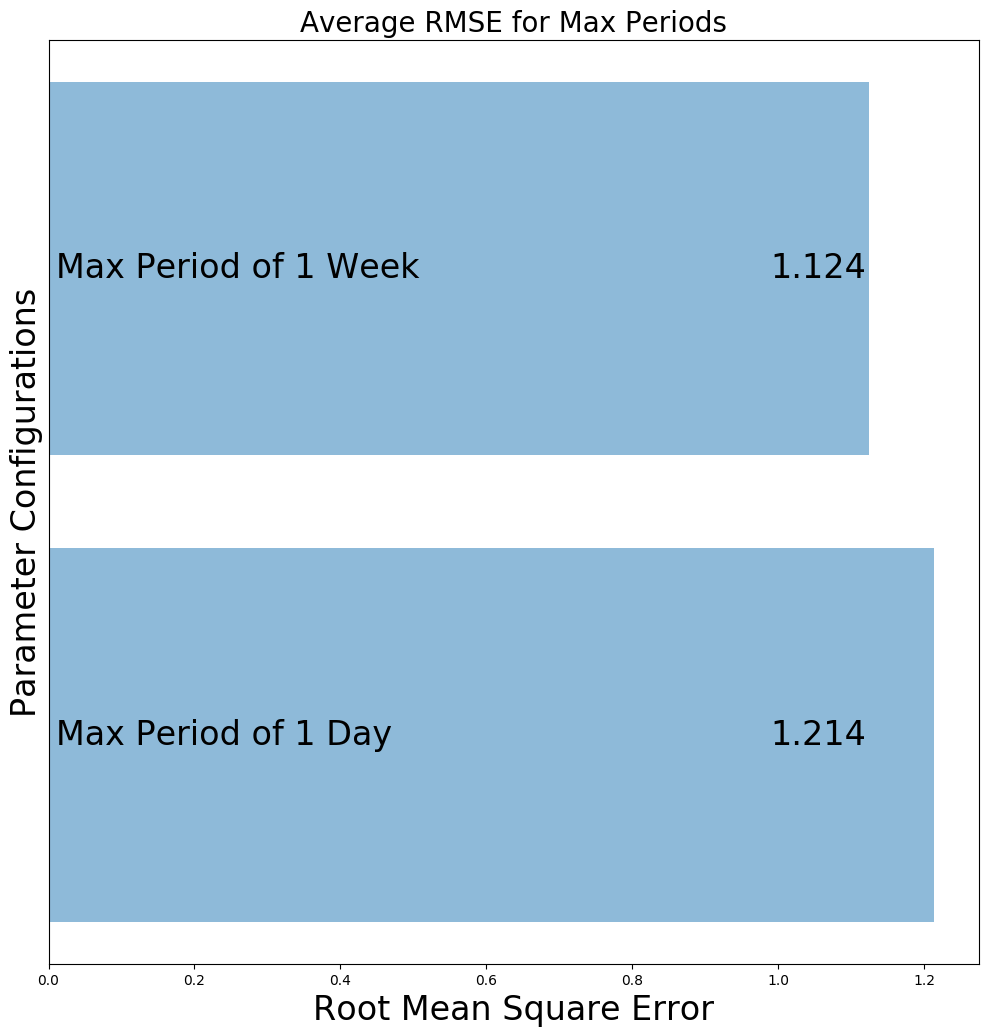
\includegraphics[width=2.3in]{images/Average_RMSE_for_Max_Periods.png}}
    {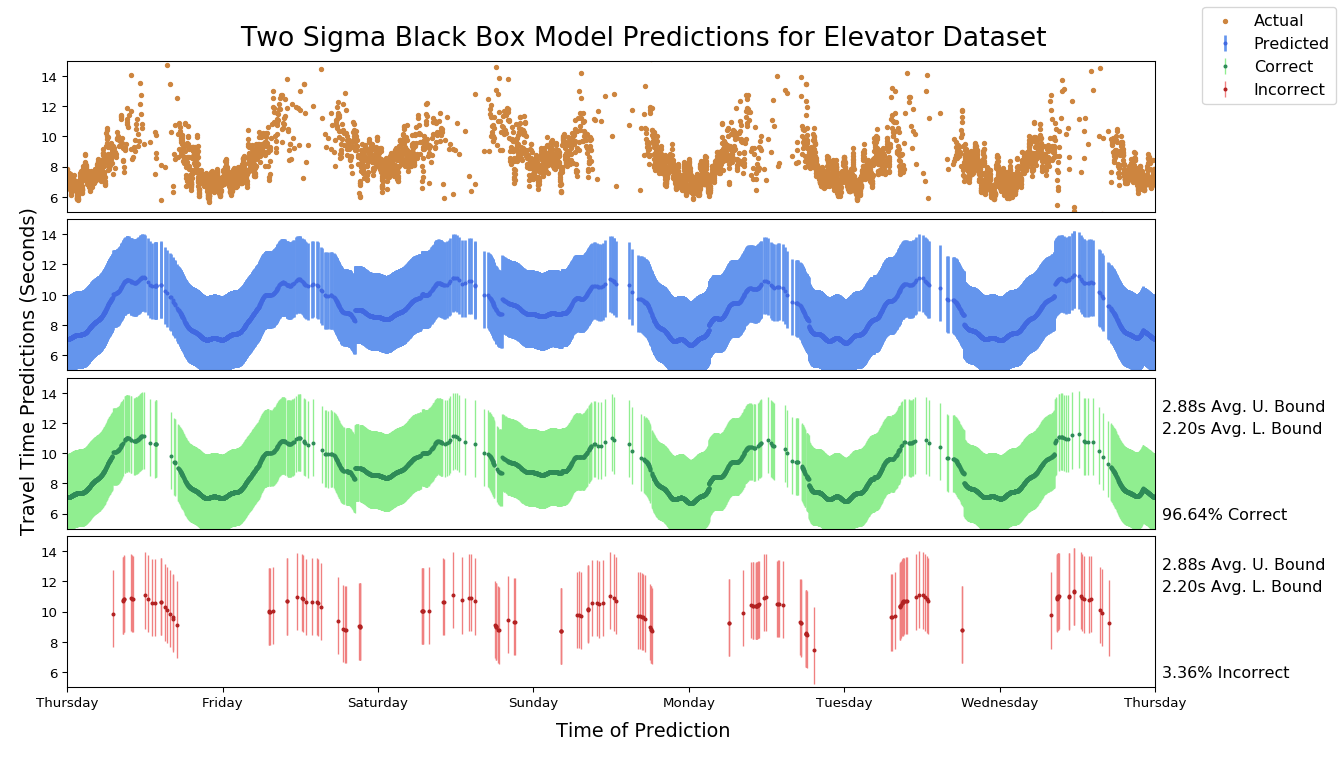
\includegraphics[width = 2.8in]{images/elevator/two_sigma_black_box_model_predictions_for_elevator_dataset.png}}

    %\column{.5\textwidth}
    %{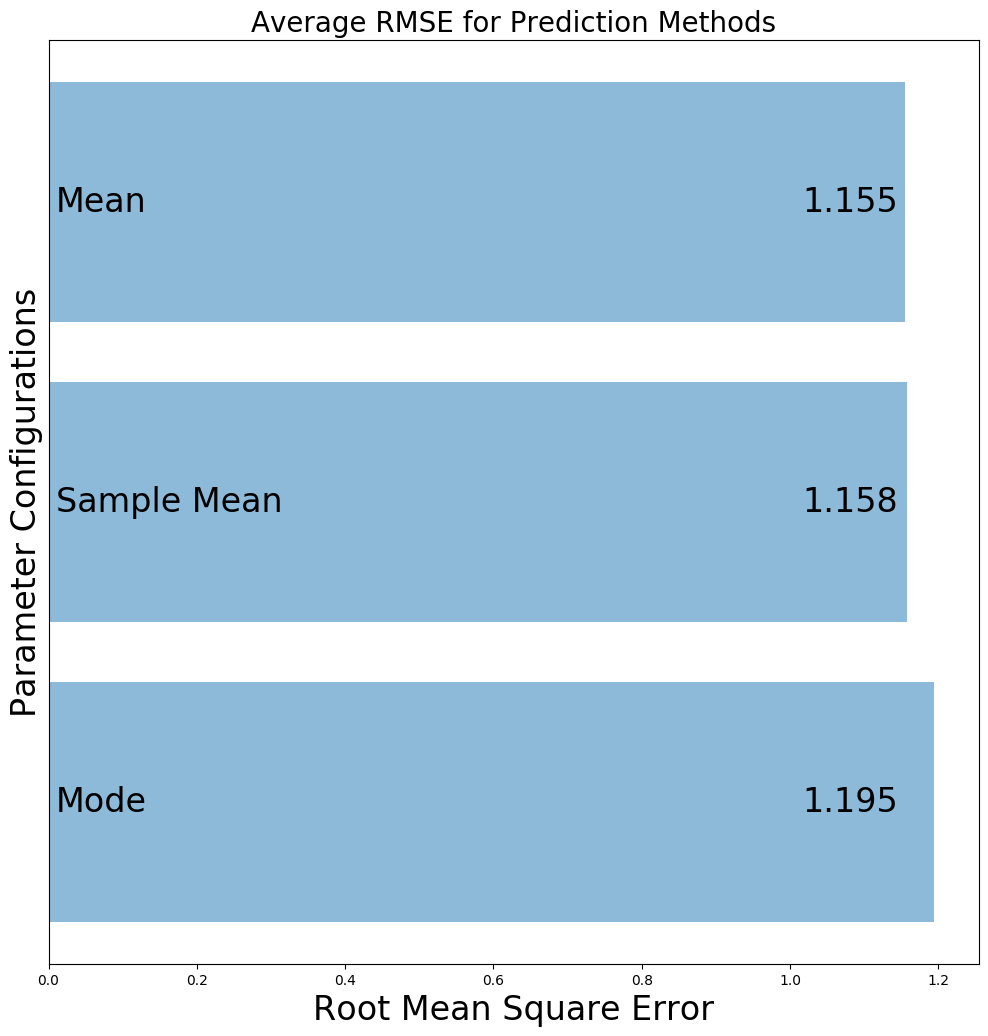
\includegraphics[width=2.3in]{images/Average_RMSE_for_Prediction_Methods.png}}
    %{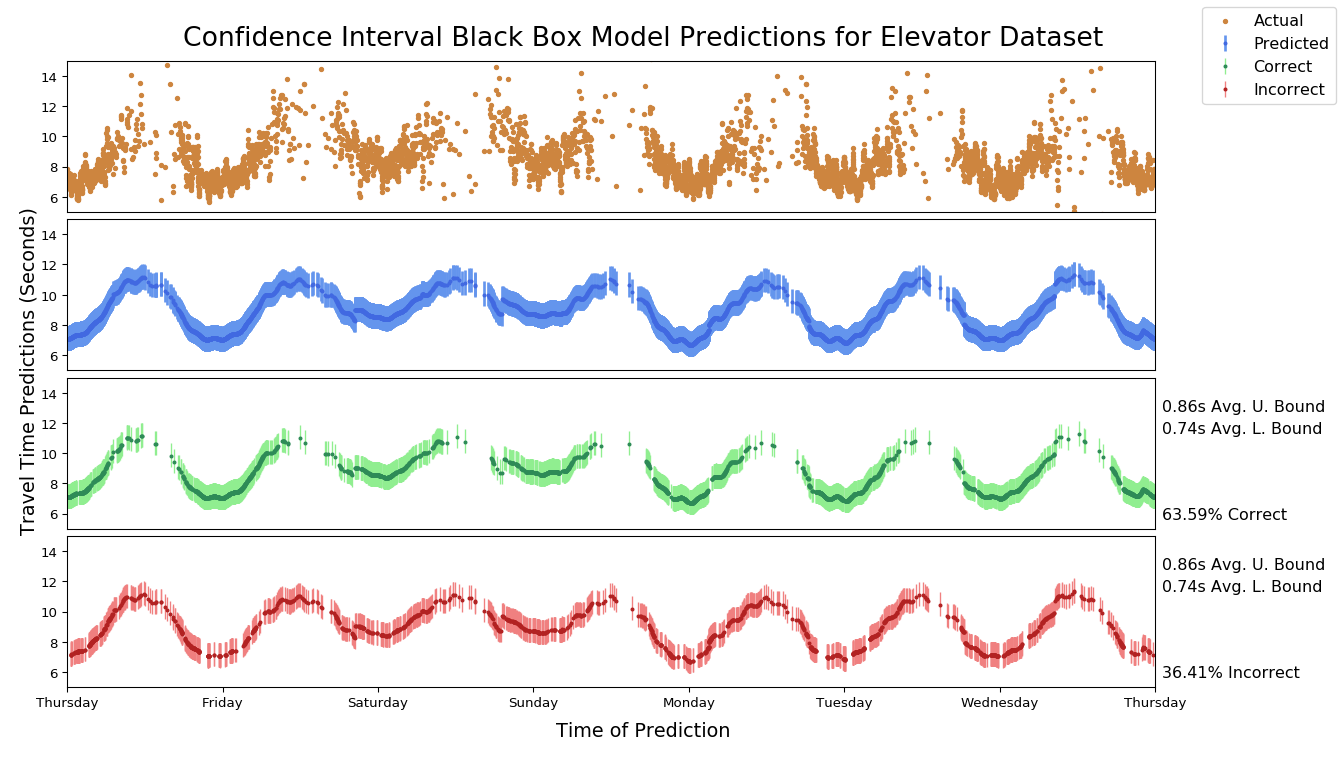
\includegraphics[width = 2.3in]{images/elevator/confidence_interval_black_box_model_predictions_for_elevator_dataset.png}}
    \begin{overlayarea}{0.5\textwidth}{0.5\textheight}


    \end{overlayarea}
  \end{columns}
  \vspace*{-0.3cm}

  \begin{columns}[t]
    %\column{.5\textwidth}
    %{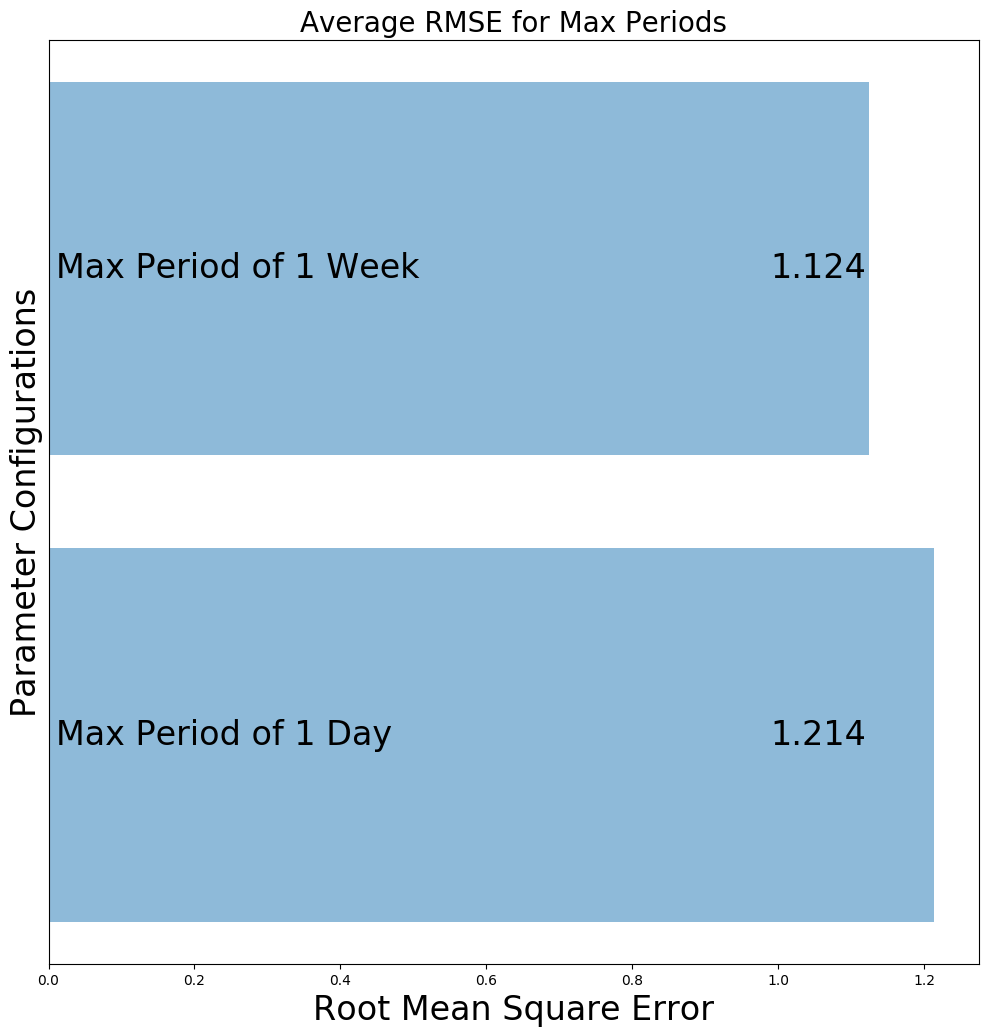
\includegraphics[width=2.3in]{images/Average_RMSE_for_Max_Periods.png}}
    %{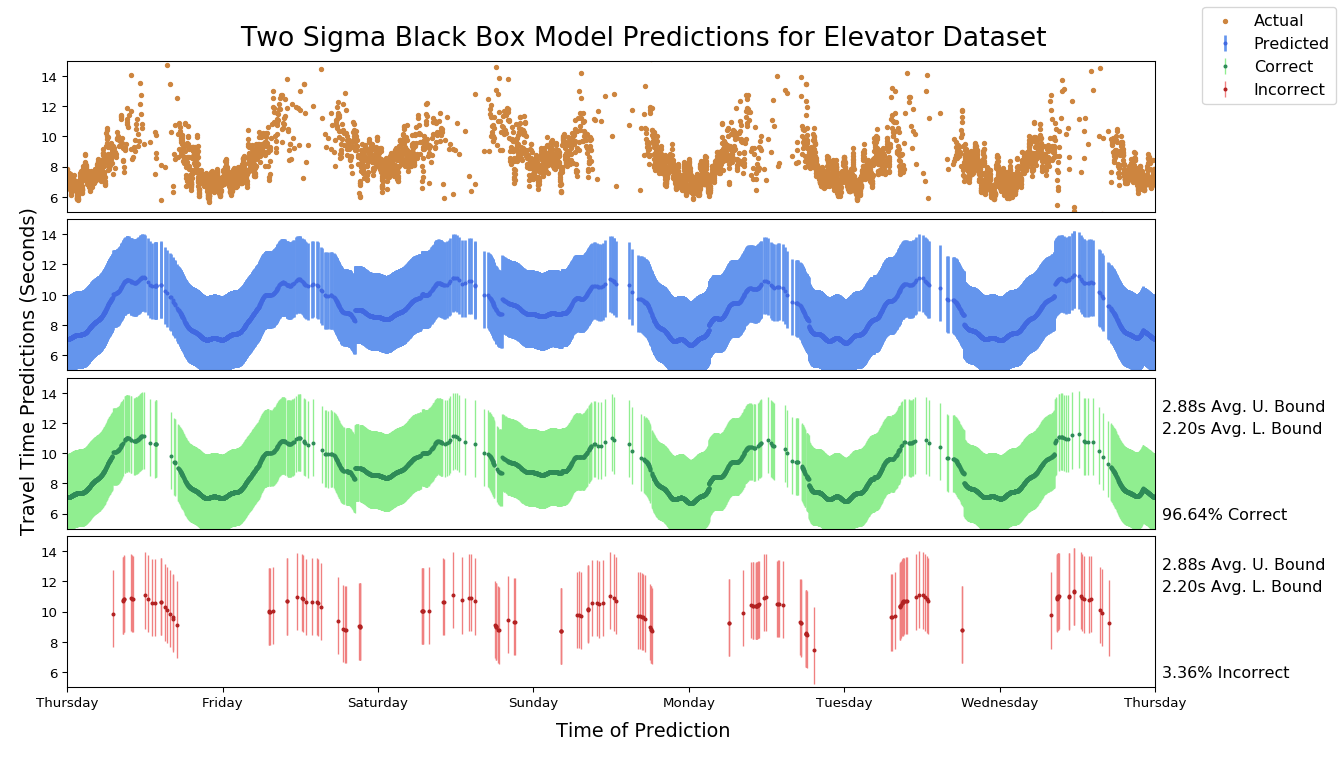
\includegraphics[width = 2.3in]{images/elevator/two_sigma_black_box_model_predictions_for_elevator_dataset.png}}

    %\column{.5\textwidth}
    %{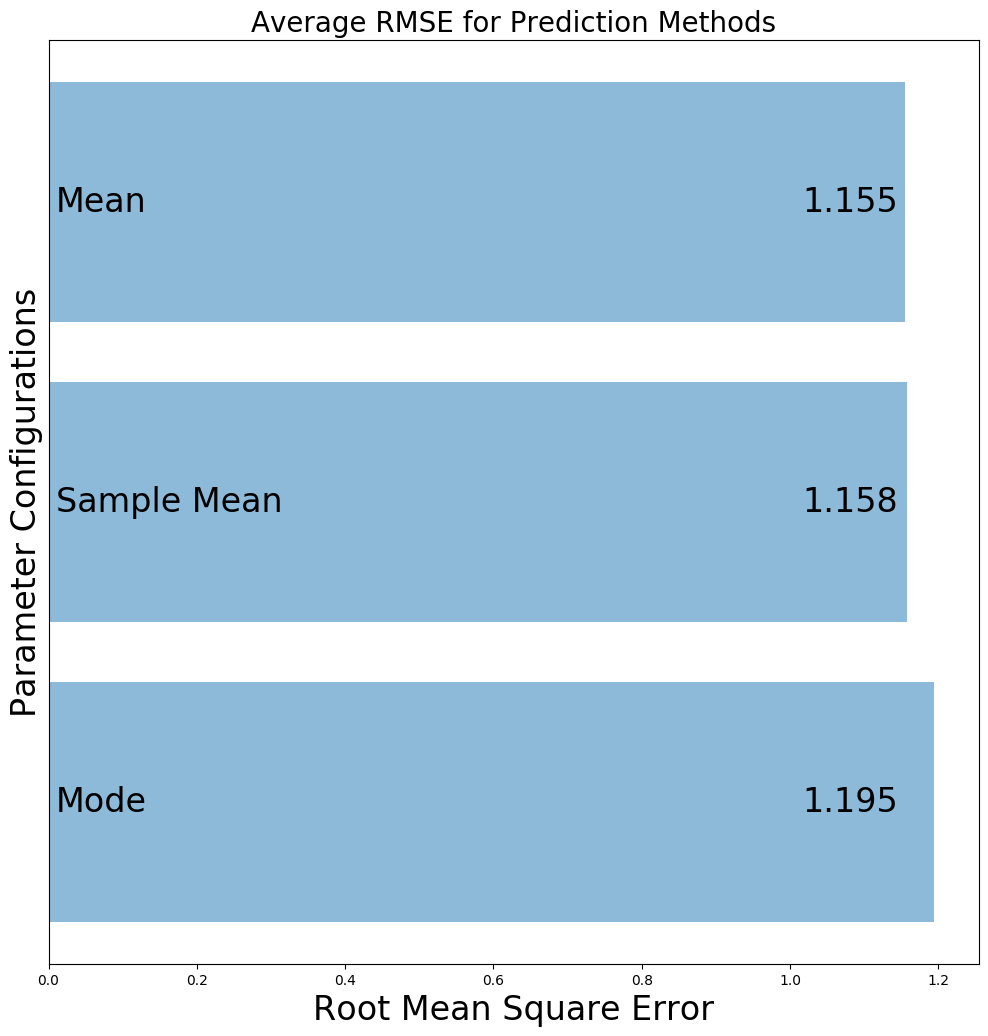
\includegraphics[width=2.3in]{images/Average_RMSE_for_Prediction_Methods.png}}
    {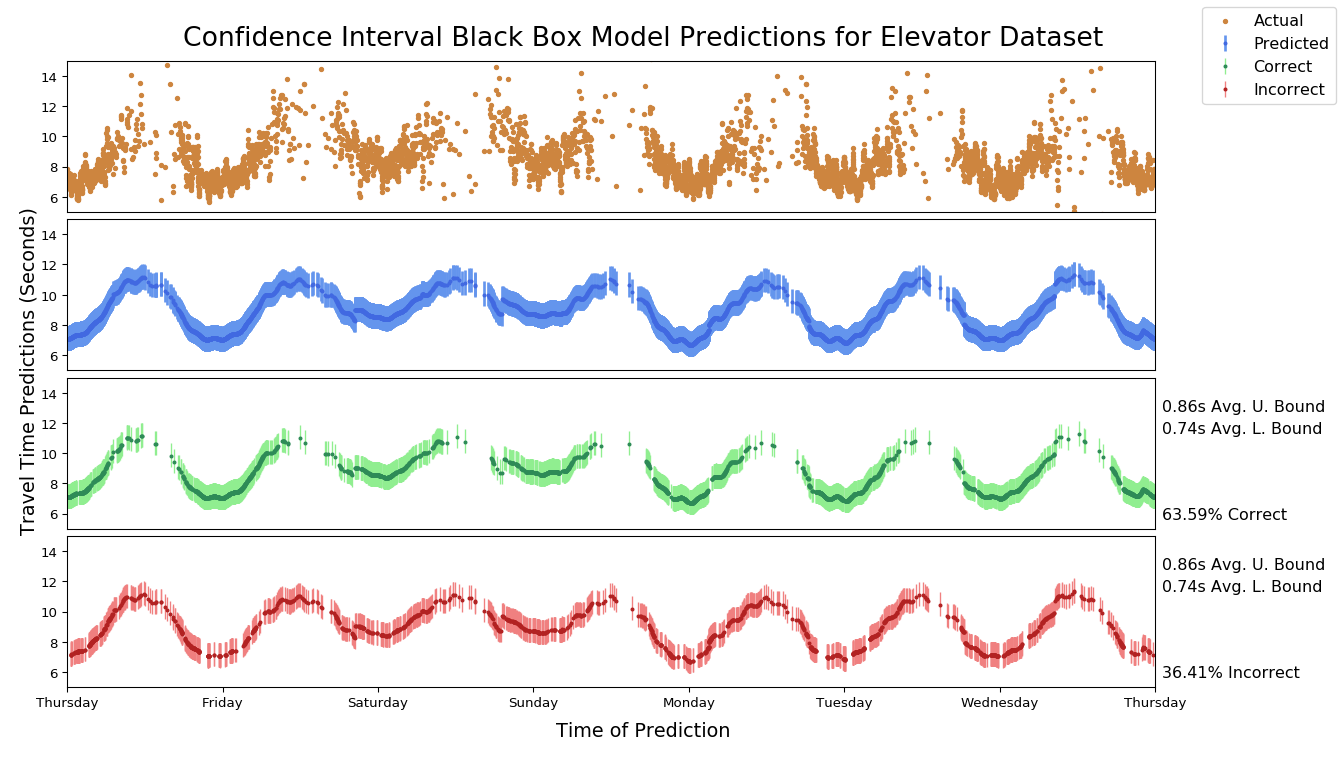
\includegraphics[width = 2.8in]{images/elevator/confidence_interval_black_box_model_predictions_for_elevator_dataset.png}}
  \end{columns}

\end{frame}



\begin{frame}[t]{Complete Elevator Dataset - Grouping}
  %\framesubtitle{Bounding Comparision}

  \vspace*{-0.9cm}
  \begin{columns}[t]
    %\column{.5\textwidth}
    %{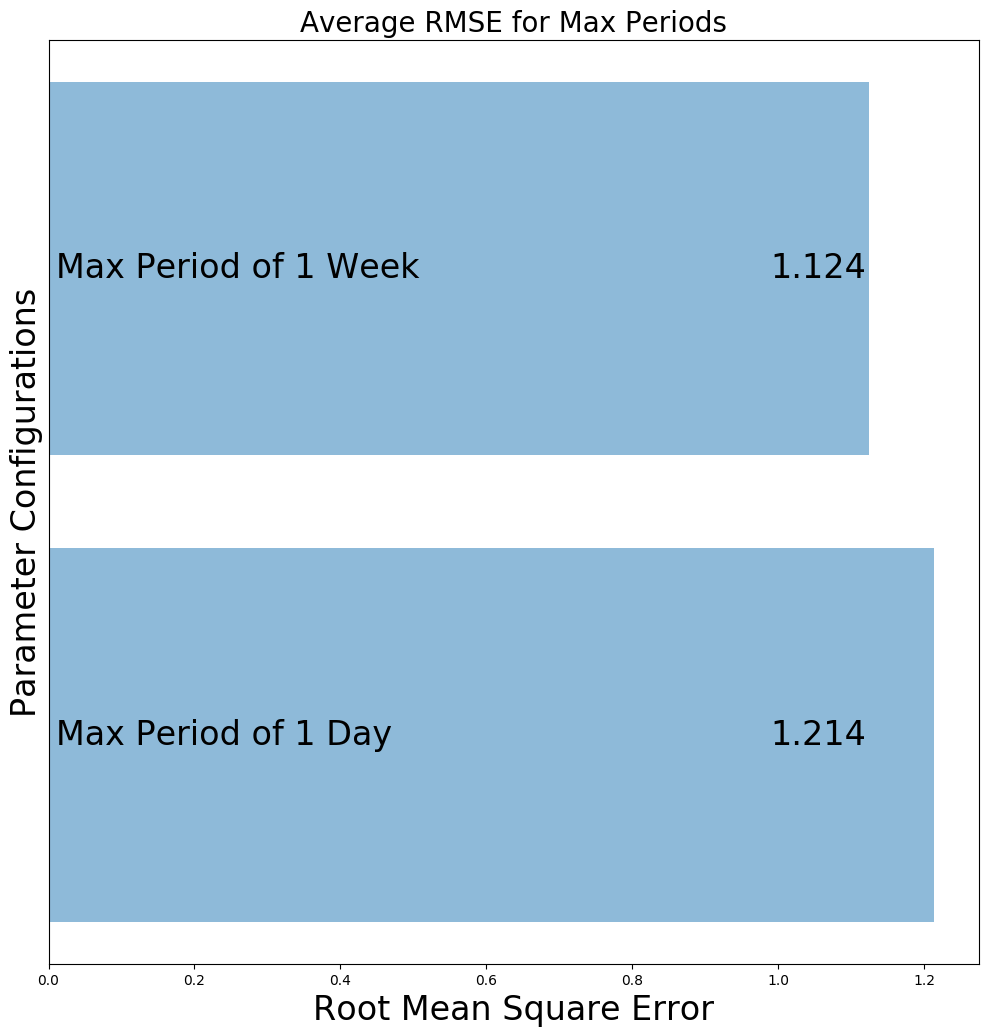
\includegraphics[width=2.3in]{images/Average_RMSE_for_Max_Periods.png}}
    {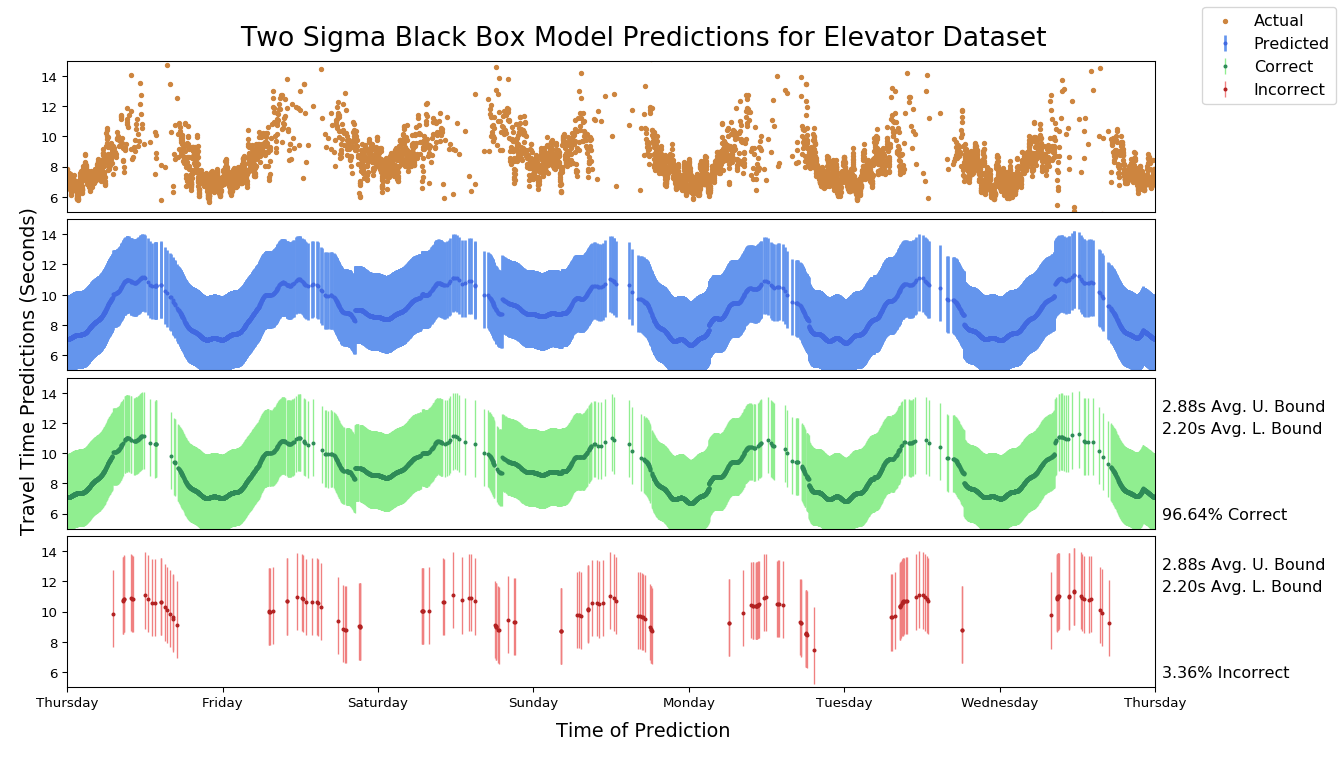
\includegraphics[width = 2.8in]{images/elevator/two_sigma_black_box_model_predictions_for_elevator_dataset.png}}

    %\column{.5\textwidth}
    %{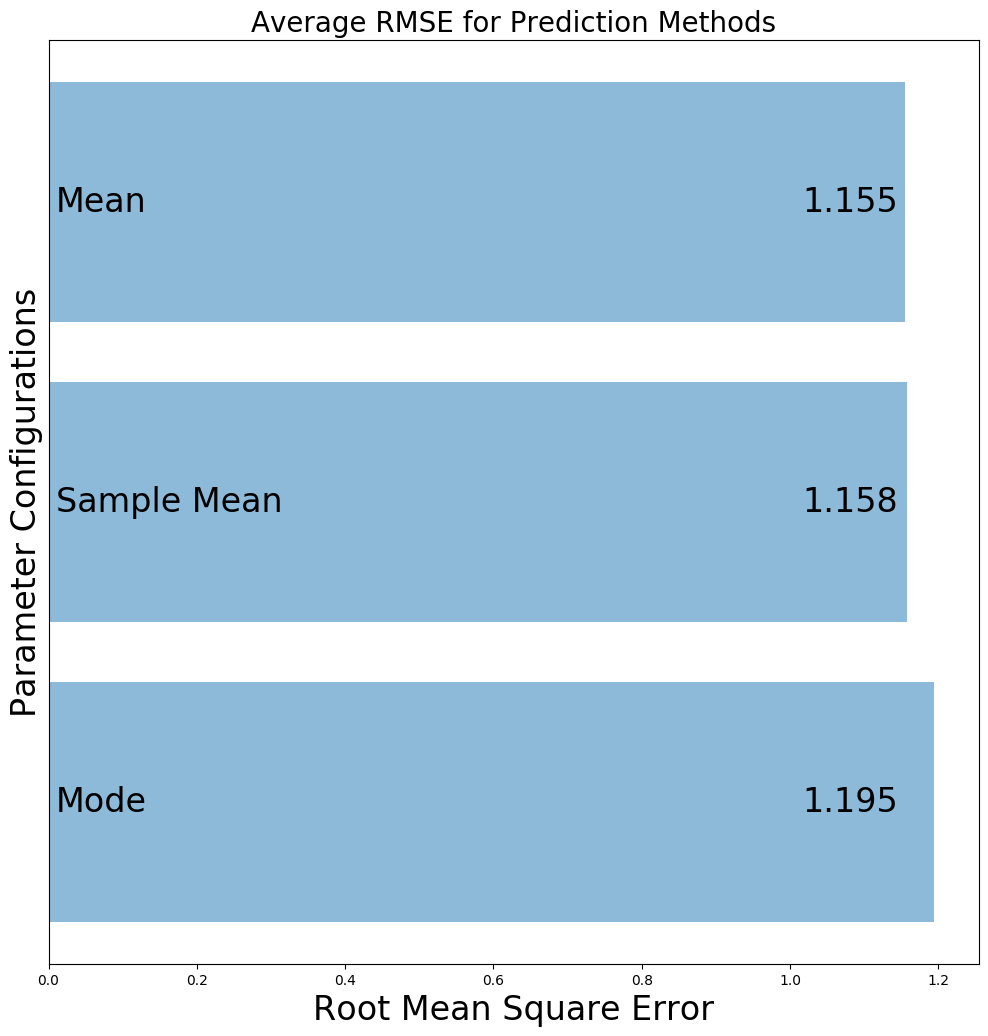
\includegraphics[width=2.3in]{images/Average_RMSE_for_Prediction_Methods.png}}
    %{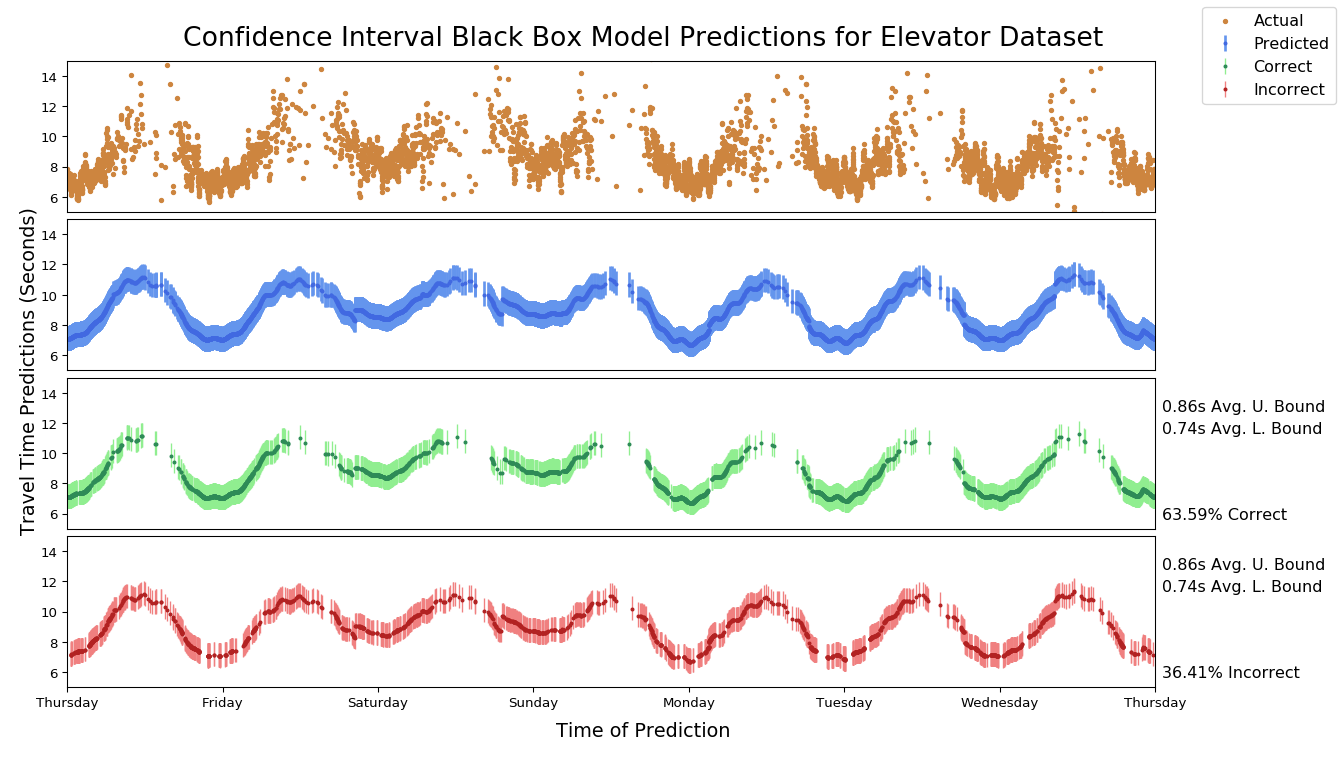
\includegraphics[width = 2.3in]{images/elevator/confidence_interval_black_box_model_predictions_for_elevator_dataset.png}}
    \begin{overlayarea}{0.5\textwidth}{0.5\textheight}


    \end{overlayarea}
  \end{columns}
  \vspace*{-0.3cm}

  \begin{columns}[t]
    %\column{.5\textwidth}
    %{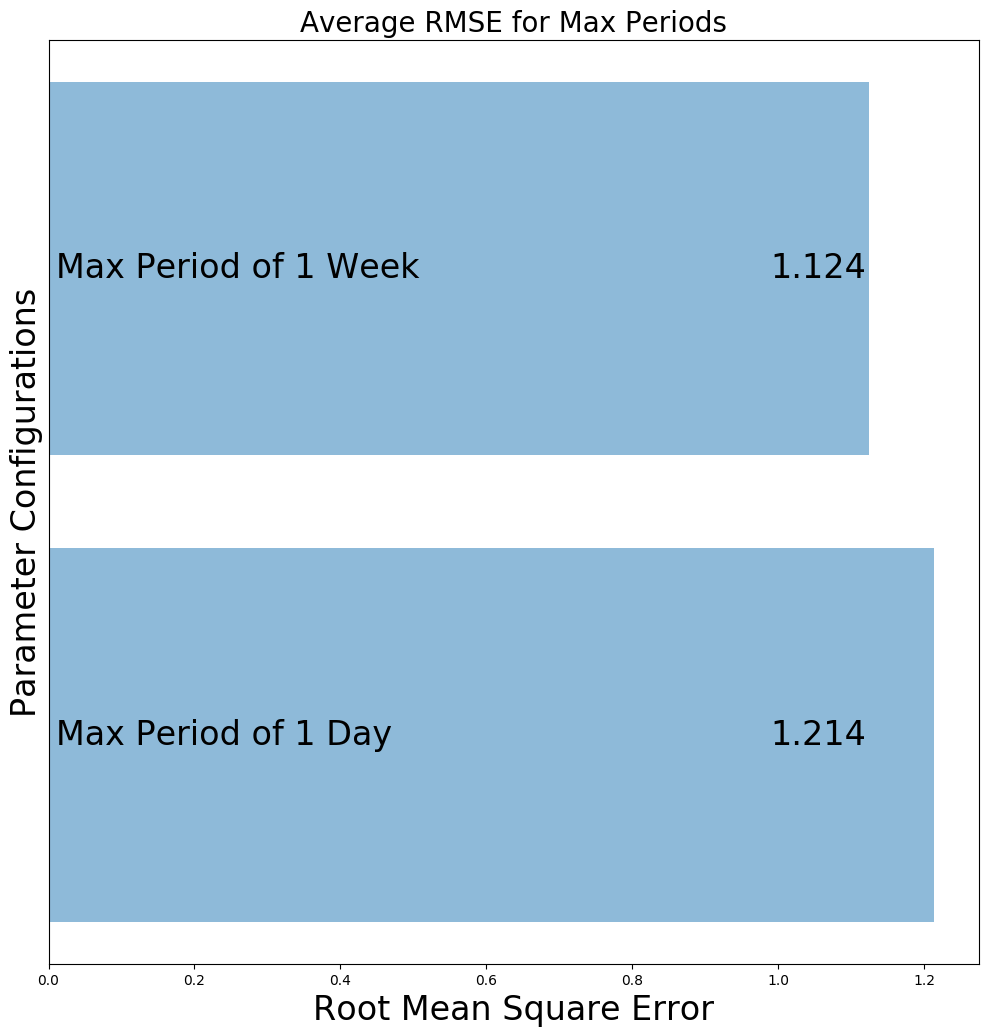
\includegraphics[width=2.3in]{images/Average_RMSE_for_Max_Periods.png}}
    %{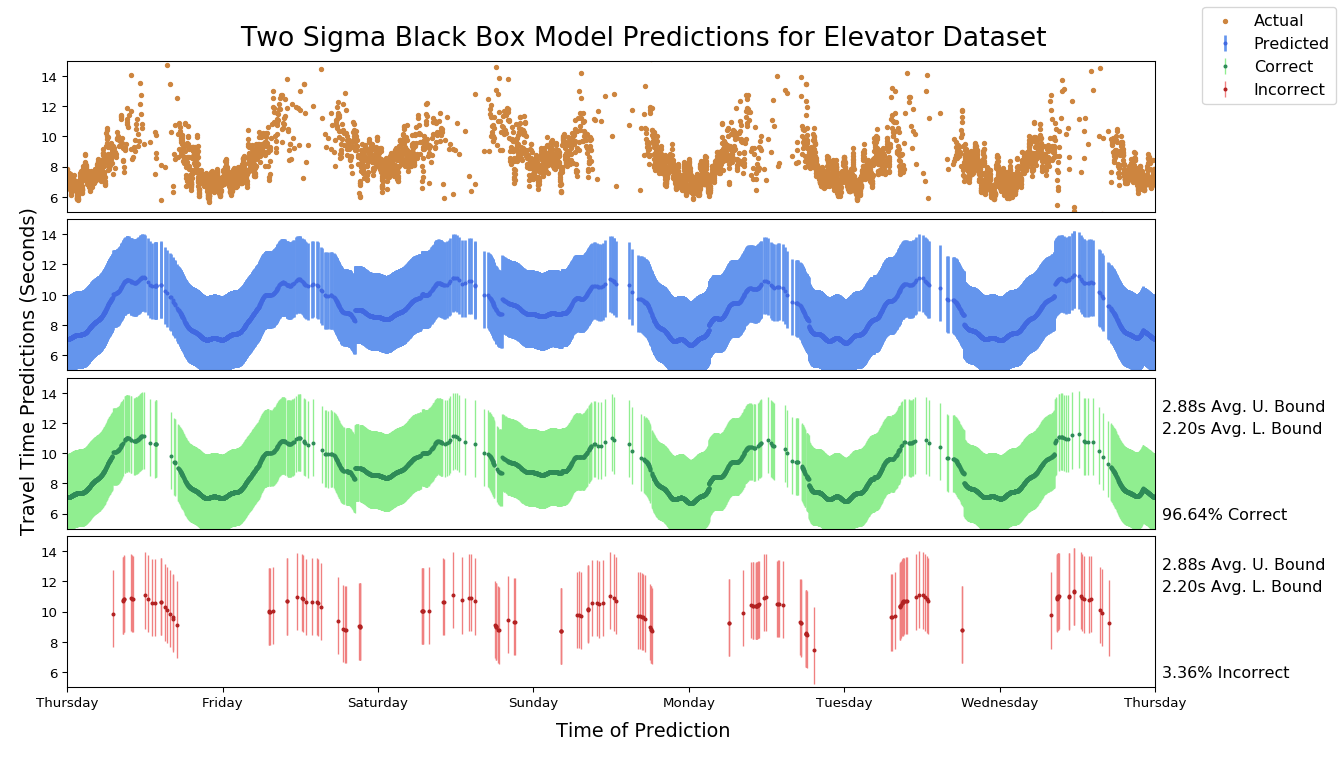
\includegraphics[width = 2.3in]{images/elevator/two_sigma_black_box_model_predictions_for_elevator_dataset.png}}

    %\column{.5\textwidth}
    %{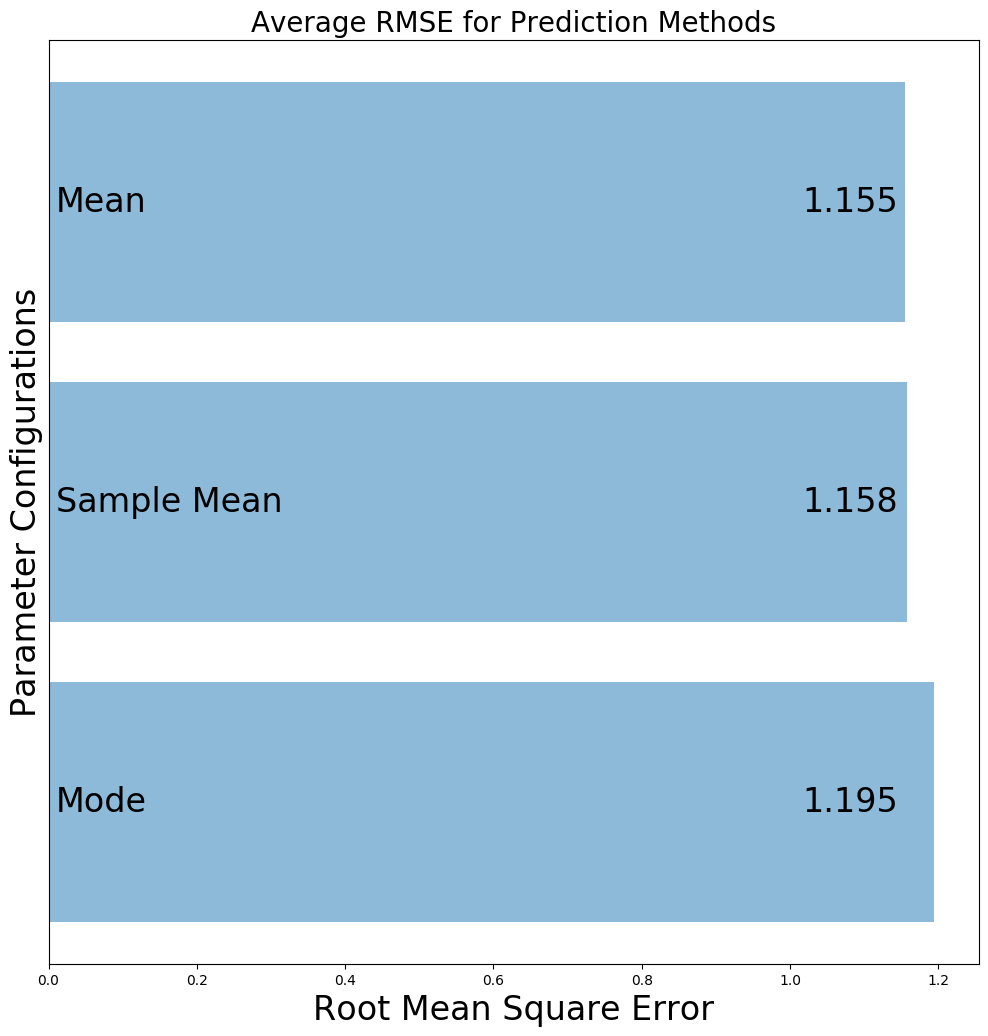
\includegraphics[width=2.3in]{images/Average_RMSE_for_Prediction_Methods.png}}
    {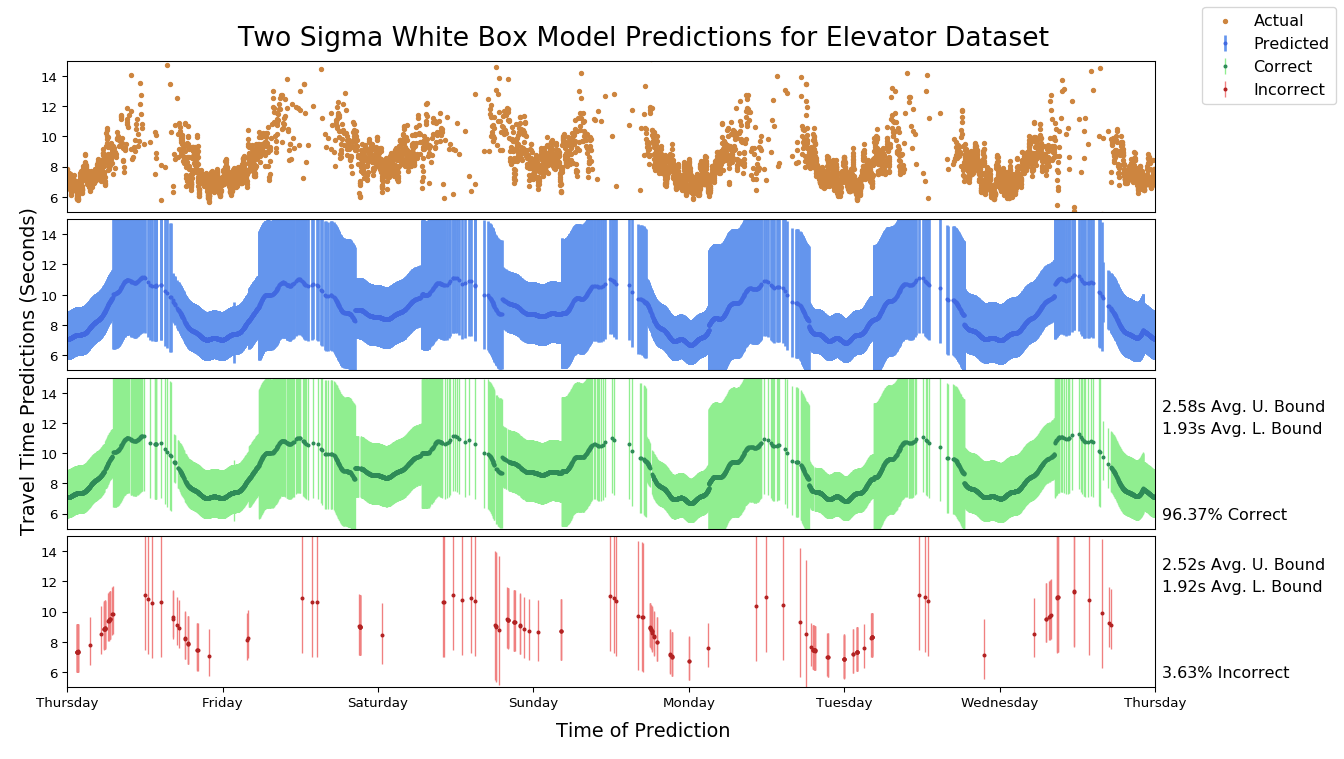
\includegraphics[width = 2.8in]{images/elevator/two_sigma_white_box_model_predictions_for_elevator_dataset.png}}
  \end{columns}

\end{frame}




\begin{frame}[t]{Sparse Elevator Dataset}
  \framesubtitle{Overall Results}

  \vspace*{-0.5cm}
  \begin{table}[htp!]
  \small
  \begin{tabular}{|p{2.5cm}|p{1.3cm}|p{1.0cm}|p{1.7cm}|p{1.0cm}|p{1.5cm}|}

    \hline
    \textbf{Model} &
    \textbf{\% Corr.} &
    \textbf{RMSE Corr.} &
    \textbf{Magnitue of Inac.} &
    \textbf{Avg. Bound} &
    \textbf{\% Invalid} \\
    \hline

    2$\sigma$ Black Box &
    93.88\% &
    1.131 &
    0.511 &
    6.347 &
    0.00\% \\
    \hline

    2$\sigma$ Grey Box &
    64.38\% &
    0.808 &
    0.913 &
    2.988 &
    17.36\% \\
    \hline

    2$\sigma$ White Box &
    89.51\% &
    1.165 &
    0.404 &
    5.346 &
    0.00\% \\
    \hline

    2$\sigma$ White X Grey Box &
    41.70\% &
    0.603 &
    1.201 &
    1.531 &
    52.99\% \\
    \hline

    CI Black Box &
    63.05\% &
    0.511 &
    0.974 &
    2.405 &
    0.00\% \\
    \hline

    CI Grey Box &
    52.70\% &
    0.627 &
    0.997 &
    2.212 &
    17.36\% \\
    \hline

    CI White Box &
    65.35\% &
    0.674 &
    0.756 &
    2.757 &
    0.00\% \\
    \hline

    CI White X Grey Box &
    37.99\% &
    0.555 &
    1.212 &
    1.353 &
    52.99\% \\
    \hline


\end{tabular}
\end{table}

\end{frame}



\begin{frame}[t]{Complete Elevator Dataset}
  \framesubtitle{Inavlid Predictions}

  %\vspace*{-0.9cm}
  {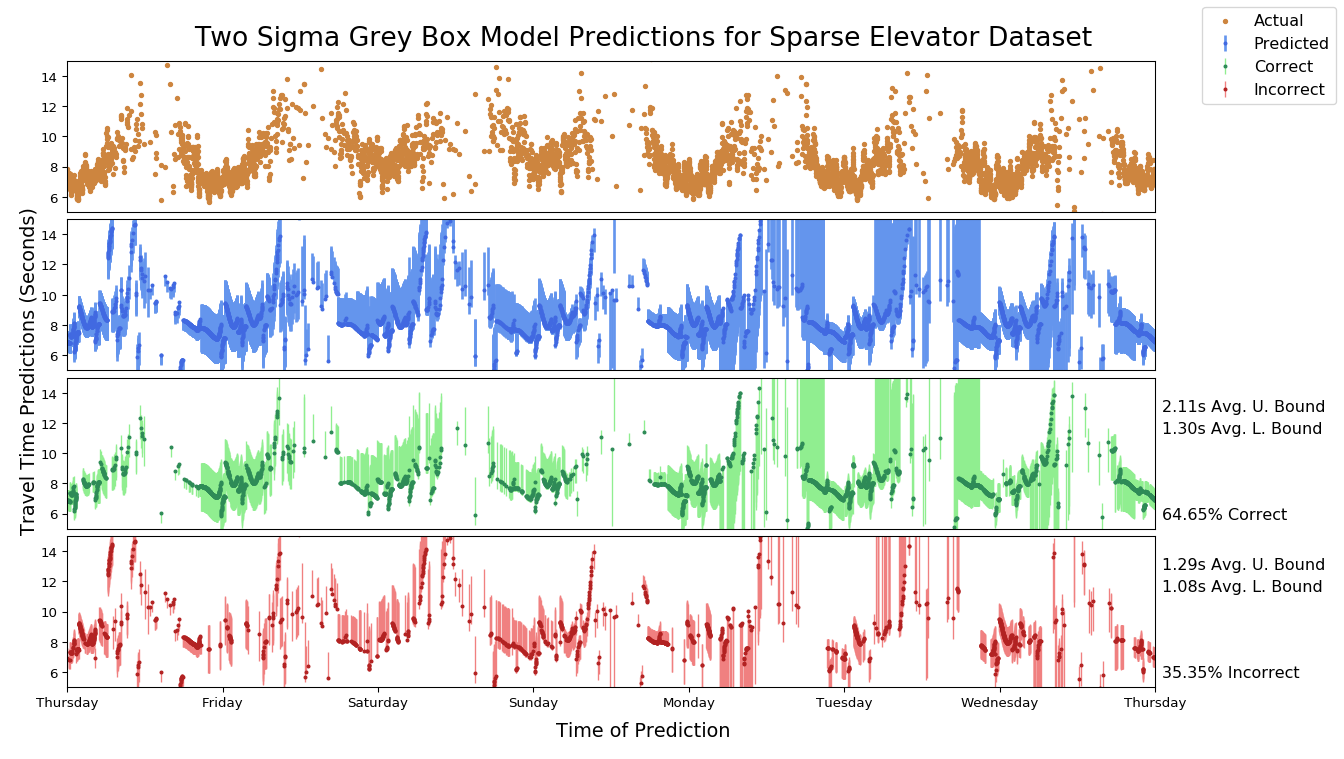
\includegraphics[width = 4.5in]{images/elevator/two_sigma_grey_box_model_predictions_for_sparse_elevator_dataset.png}}

\end{frame}



\begin{frame}[t]{Doors Experiment}
  \framesubtitle{Results: C - Permanent Change}
  {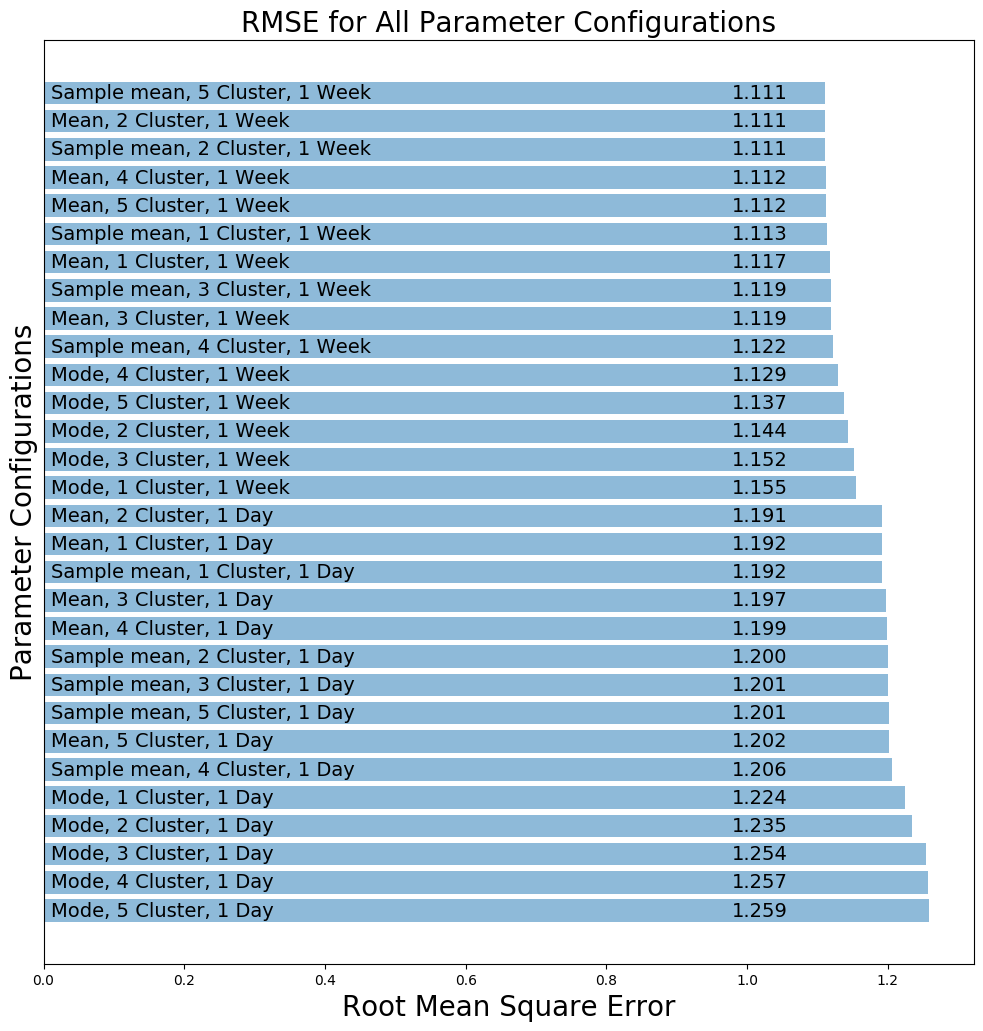
\includegraphics[width = 4.5in]{images/RMSE_for_All_Parameter_Configurations.png}}

  \begin{table}[h!]
    \centering
    \resizebox{\textwidth}{!}{%
      \begin{tabular}{|l|l|l|l|l|}
        \hline
        & DMM & Gaussian & FreMEn  & Hypertime \\ \hline
        Prediction Accuracy             & 31.82\% & 14.58\%  & 00.00\% & 00.00\%   \\ \hline
        Computation Time (Milliseconds) & 570     & 60       & 70      & 530       \\ \hline
        Memory Usage (KB)               & 31224   & 35004    & 34976   & 37208     \\ \hline
      \end{tabular}%
    }
  \end{table}

\end{frame}


\begin{frame}[t]{Congested Hallways}
  \framesubtitle{Navigation with a Graph}
  \begin{itemize}
    \setlength\itemsep{.5em}
    \item Uses binary predictions for path planning
    \item Goal is to move from Start to Finish during different times
    \item Consists of 7 nodes with dynamic behavior
    \begin{itemize}
      \item 2 Meal Nodes - three times a day
      \item 1 Laundry Node - once per day
      \item 2 Delivery Nodes - twice per week
      \item 2 Trash Nodes - once every three days
    \end{itemize}
  \item Path planning done with NetworkX
  \item Metrics
  \begin{itemize}
    \item Hard vs Soft Errors
    \item Additional Travel Distance
  \end{itemize}

  \end{itemize}
\end{frame}

\begin{frame}[t]{Congested Hallways}
  \vspace*{-2cm}


  \begin{figure}
    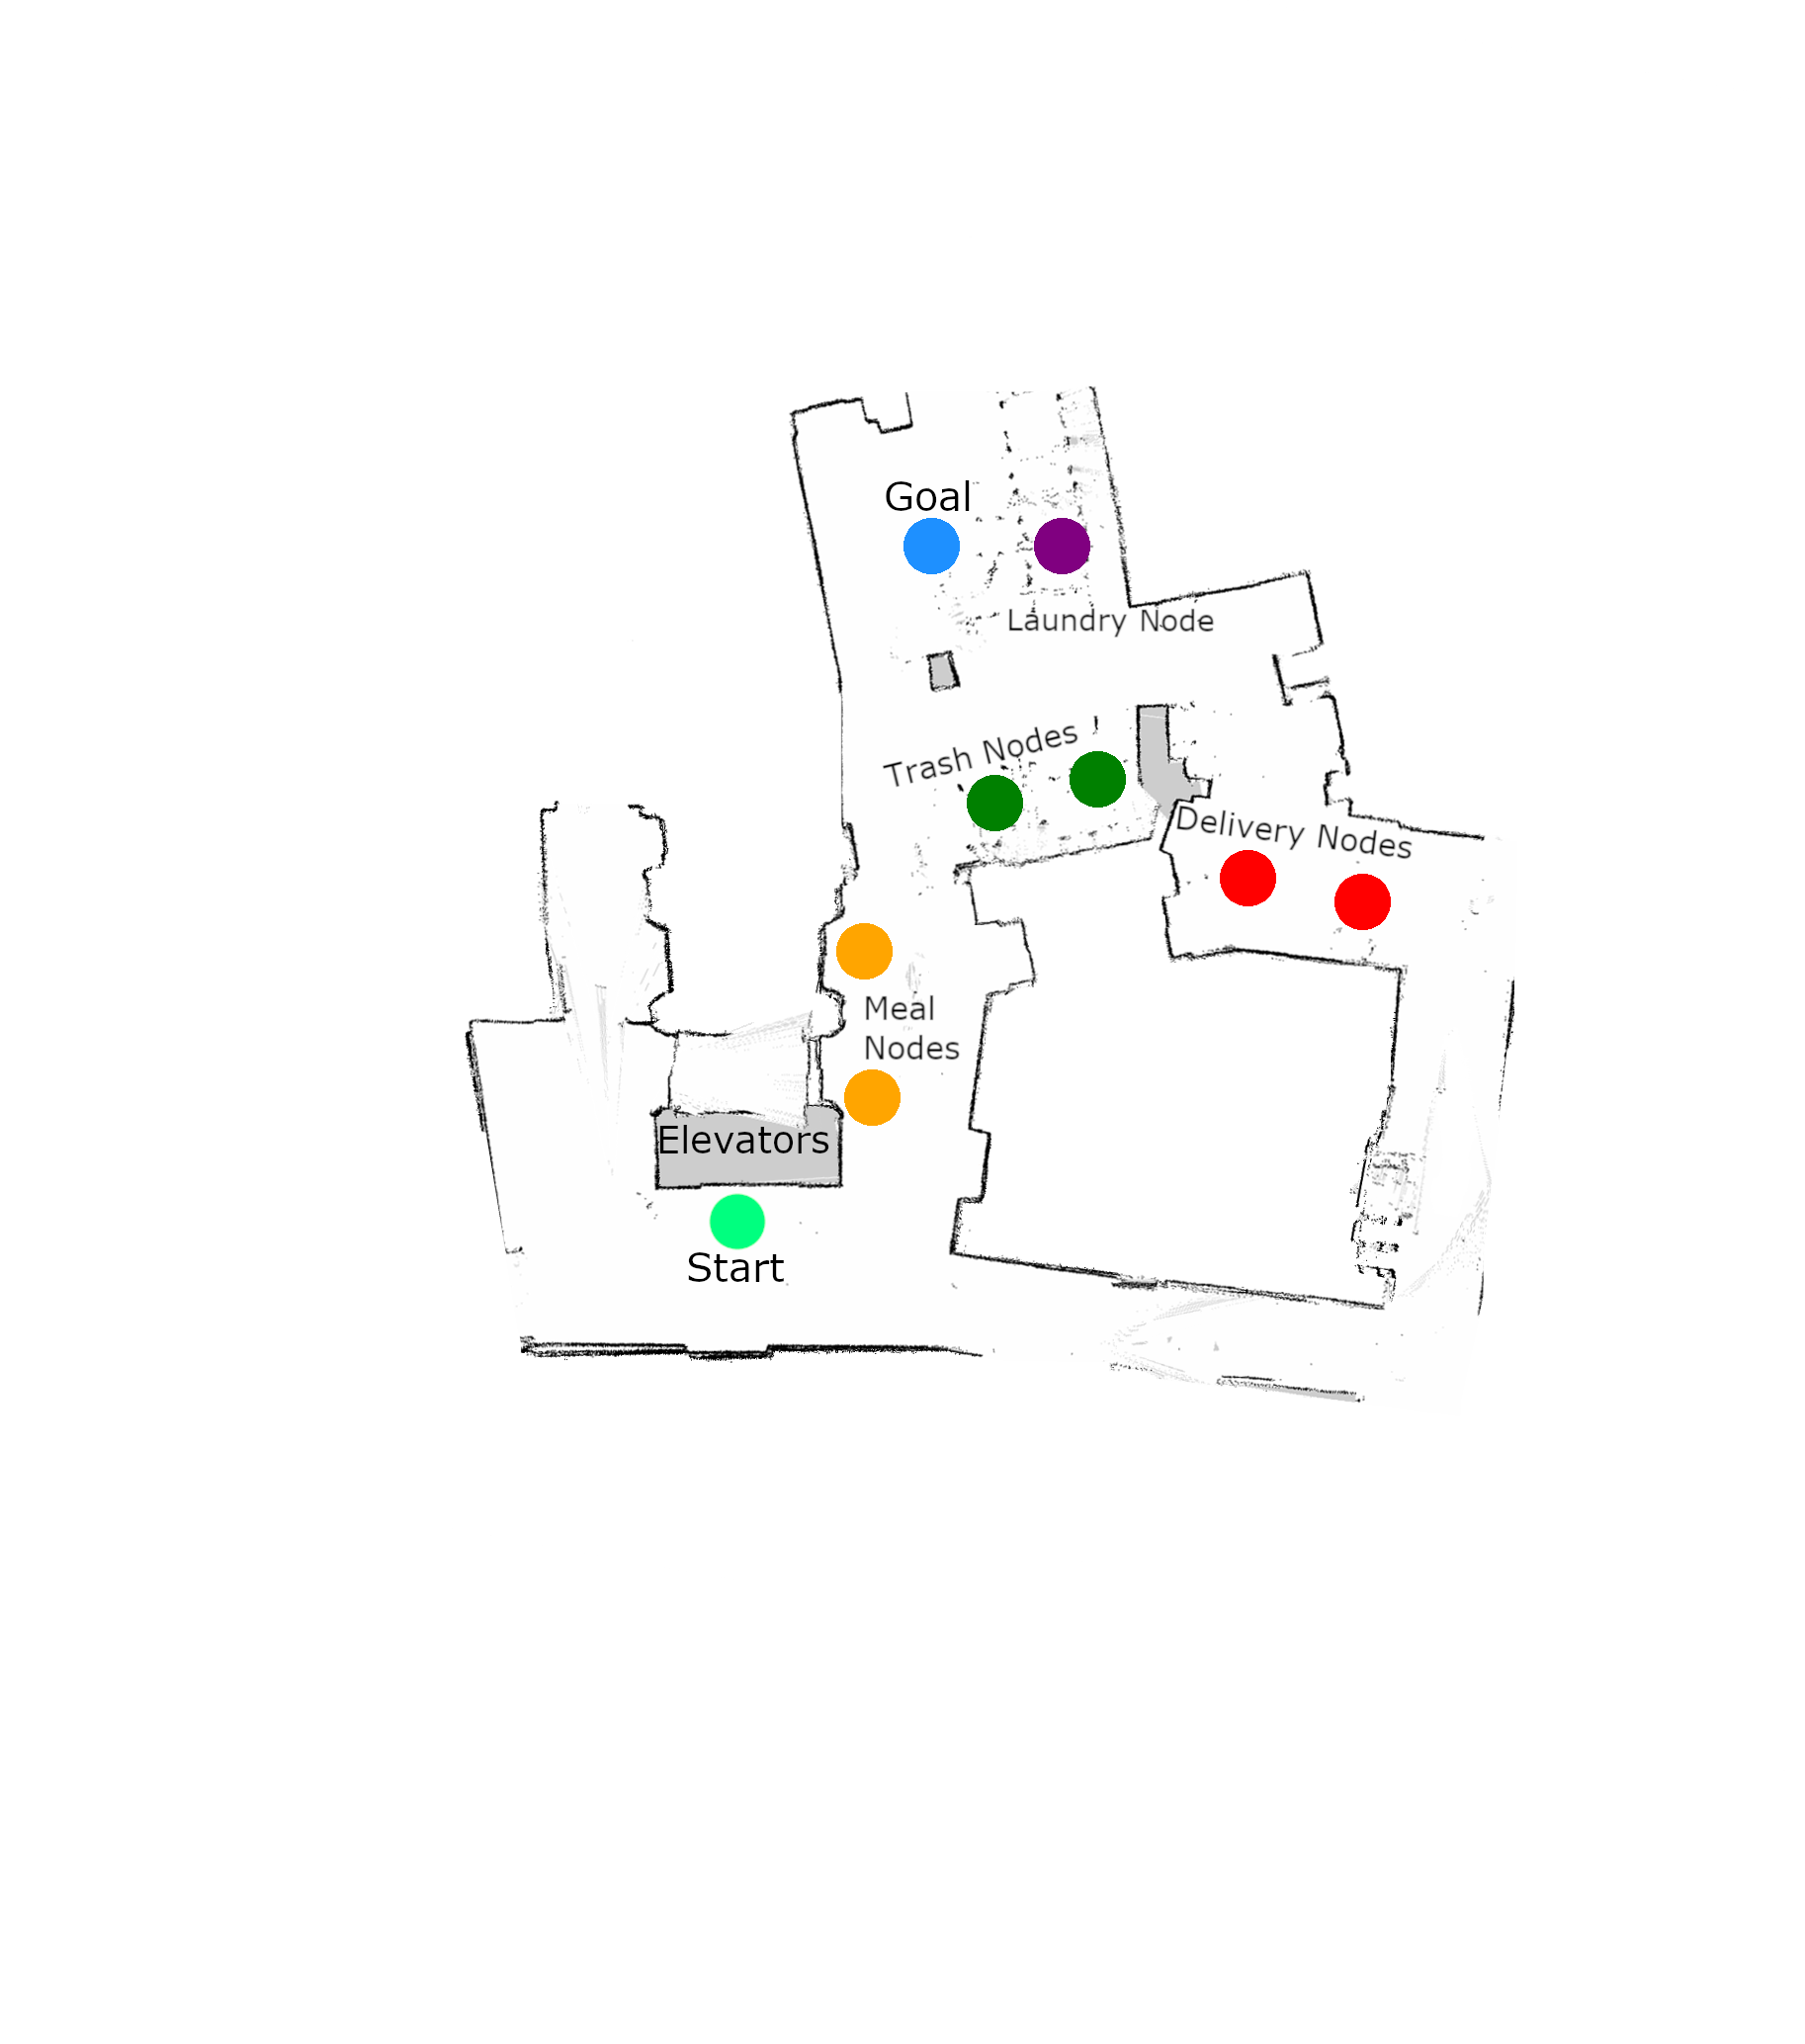
\includegraphics[width=2.5in]{images/results/overlay.png}
    %\caption{Layout}
    \vspace*{-2.5cm} % remove spacing between figure and caption
  \end{figure}

  \vspace*{-.75cm} % remove spacing between figures
  \begin{columns}[T]
    \begin{column}{0.5\textwidth}
      \begin{figure}
        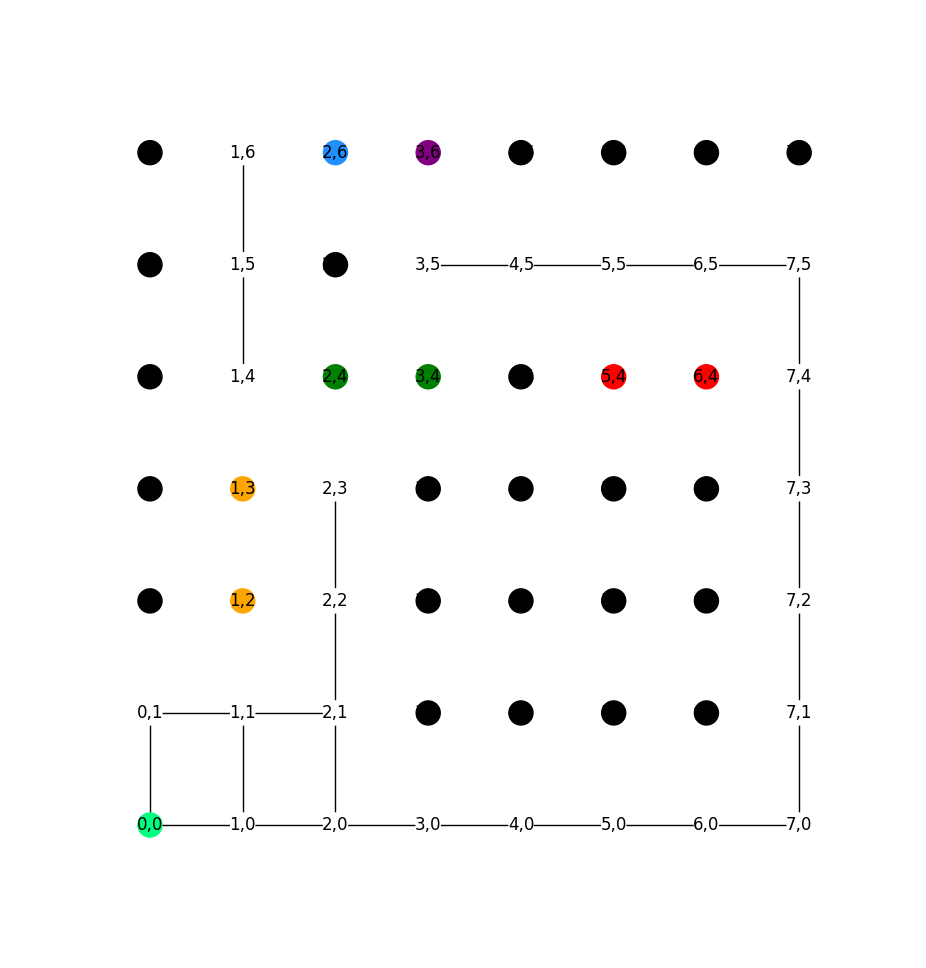
\includegraphics[width=1.75in]{images/results/Full_Hospital.png}
        \vspace*{-0.3cm}
        %\caption{Example B}
      \end{figure}
    \end{column}

    \begin{column}{0.5\textwidth}
      \begin{figure}
        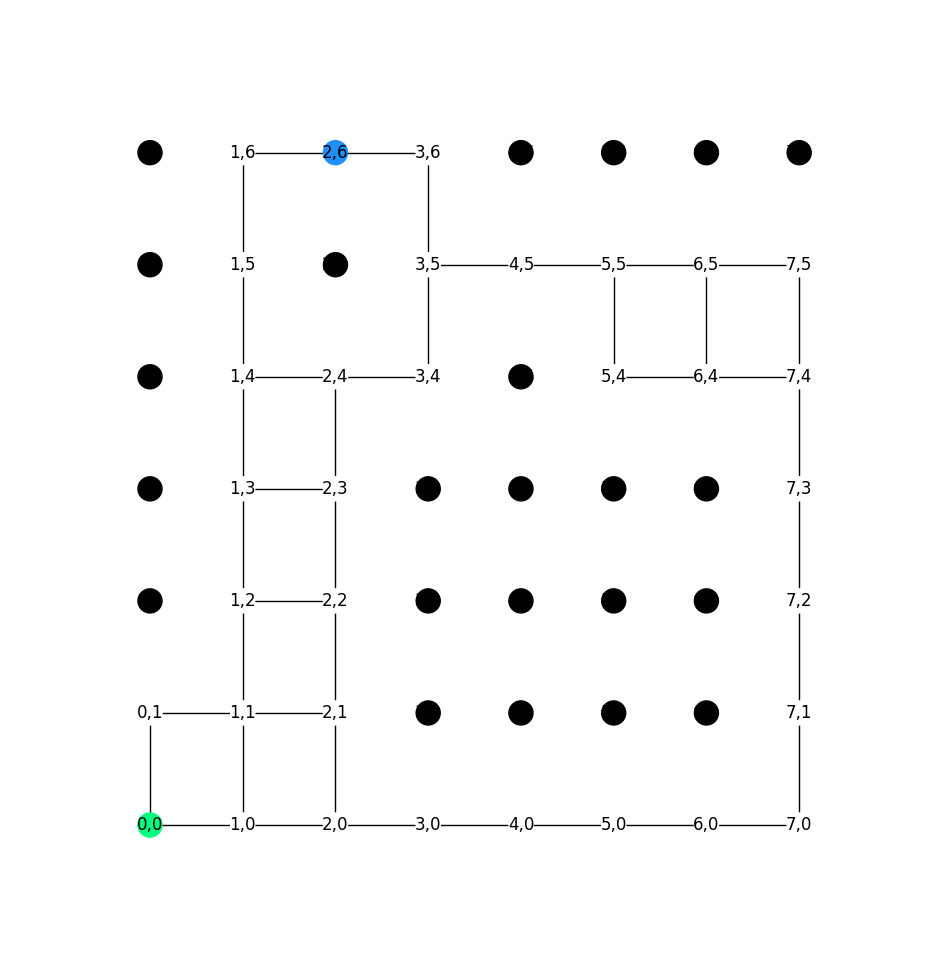
\includegraphics[width=1.75in]{images/results/Empty_Hospital.png}
        \vspace*{-0.3cm}
        %\caption{Example C}
      \end{figure}
    \end{column}
  \end{columns}

\end{frame}


\begin{frame}[t]{Congested Hallways}
  \framesubtitle{Overall Results}

  \vspace*{-0.5cm}
  \begin{table}[htb!]
    \centering
    \resizebox{\textwidth}{!}{%
      \begin{tabular}{|l|l|l|l|l|}
        \hline
        & DMM & Gaussian & FreMEn  & Hypertime \\ \hline
        Number of Hard Errors              & 1790   & 2418   & 1488   & 1488 \\ \hline
        Number of Soft Errors              & 444    & 62     & 80     & 80   \\ \hline
        Average Additional Cells Traversed & 5.74   & 6.34   & 3.12   & 3.12 \\ \hline
        Total Time Spent Planning (Milliseconds)     & 3650   & 360    & 440    & 13780\\ \hline
        Maximum Memory Usage (KB)          & 31384  & 35660  & 35588  & 38372\\ \hline
      \end{tabular}%
    }
    \caption{Future Path Planning Results}
    \label{table:Future_Path_Planning_Results}

    \begin{center}
      \begin{figure}[!hp]
        \begin{tabular}{cc}
          {\includegraphics[width = 3.75in]{images/results/future_average_distance_from_optimal_path_during_planning.png}} \\
        \end{tabular}
      \end{figure}
    \end{center}
  \end{table}

\end{frame}


\begin{frame}[t]{Congested Hallways}
\framesubtitle{Predictions on High and Low Frequency Events}
  \vspace*{-0.5cm}
\begin{figure}[!Hp]
  \begin{tabular}{cc}
    {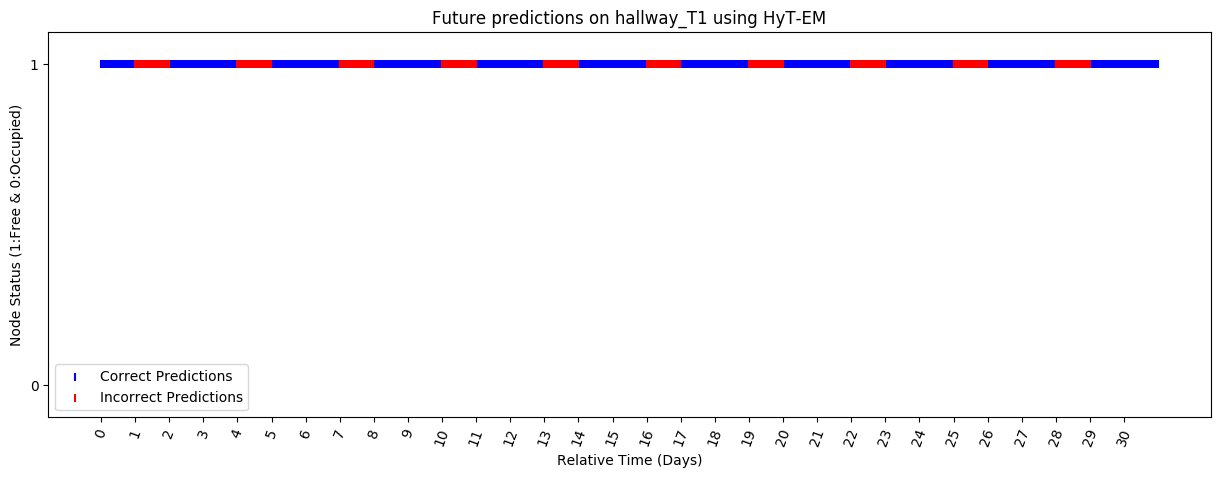
\includegraphics[width = 3.5in]{images/results/Future_hallway_T1_HyT-EM.png}} \\
    {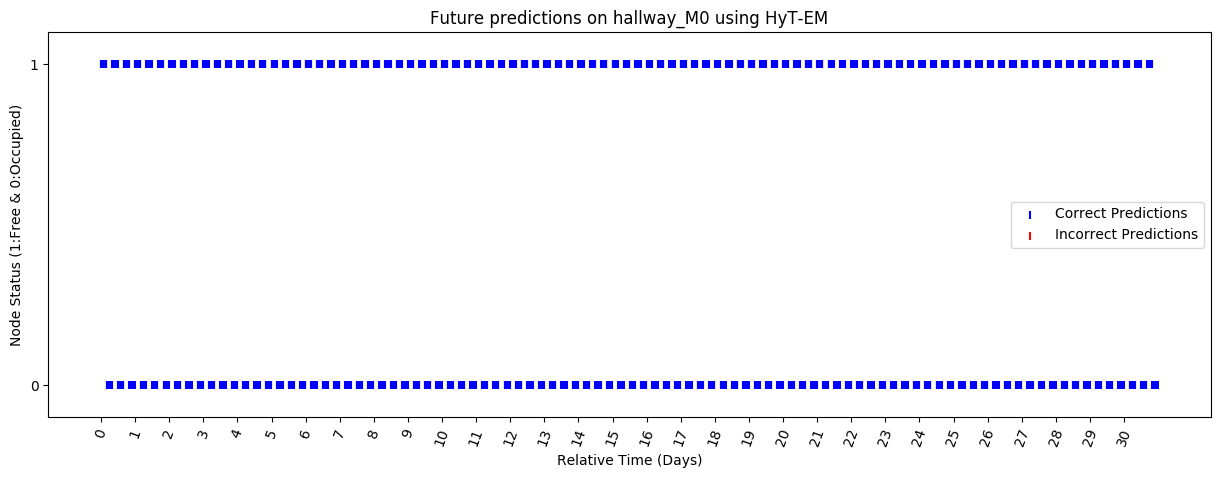
\includegraphics[width = 3.5in]{images/results/Future_hallway_M0_HyT-EM.png}} \\
  \end{tabular}
\end{figure}
\end{frame}



\begin{frame}[t]{Busy Elevator}
  \framesubtitle{Non-Binary Predictions}

  \begin{itemize}
    \setlength\itemsep{.3em}
  \item Elevator wait times vary throughout the day
  \item How far in advance should one call the elevator
  \item Test of non-binary prediction
  \begin{itemize}
    \item Binary classifiers used a fixed threshold for prediction
    \item The upper and lower averages are used for predictions
  \end{itemize}

  \begin{figure}[!htb]
    \centering
    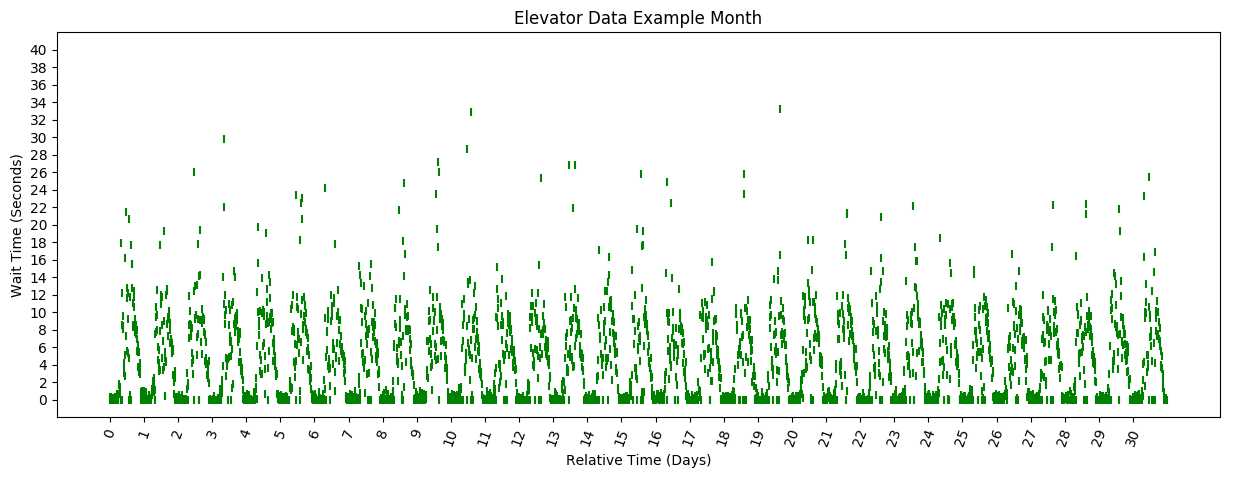
\includegraphics[width=\linewidth]{images/Elevator_Data_Example_Month.png}
  \end{figure}

  \end{itemize}
\end{frame}



\begin{frame}[t]{Busy Elevator}
 % \framesubtitle{Results}



  %\begin{figure}[!Hp]
  %  \begin{tabular}{cc}
  %    {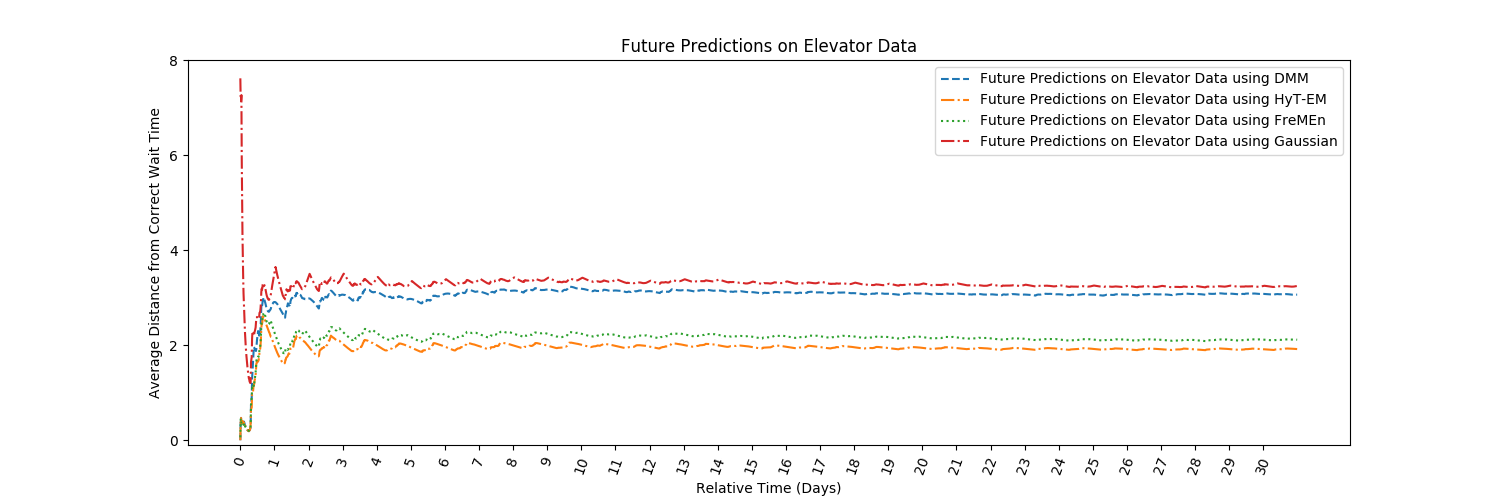
\includegraphics[width = 4.5in]{images/results/Future_Predictions_on_Elevator_Data.png}}
  %    {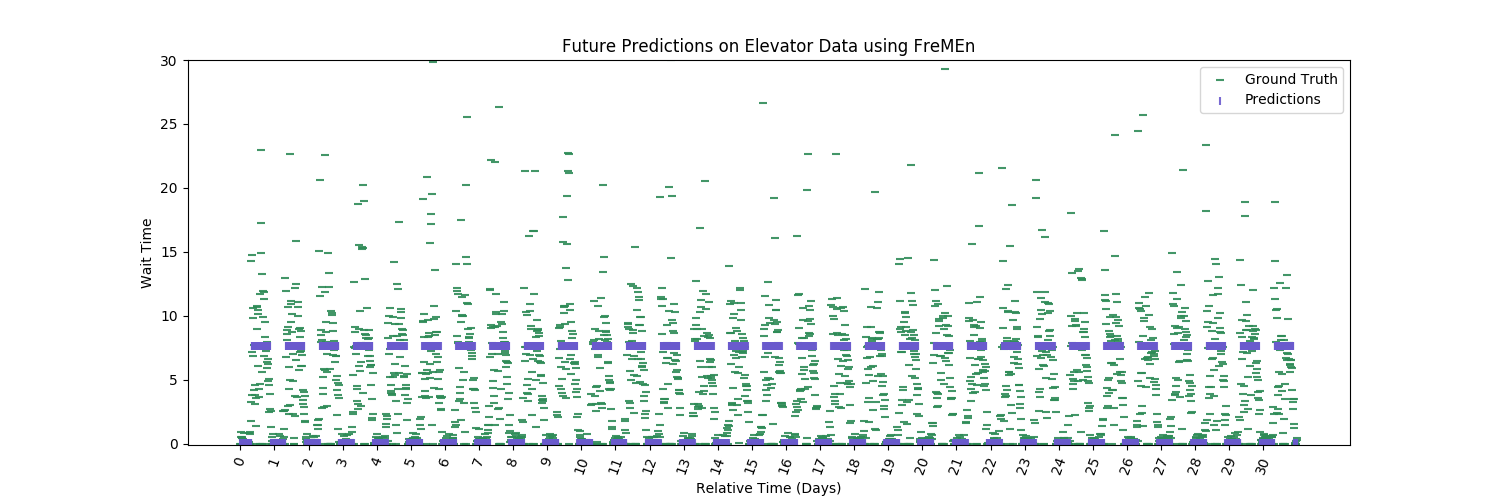
\includegraphics[width = 3in]{images/results/Future_elevator_FreMEn.png}}
  %    {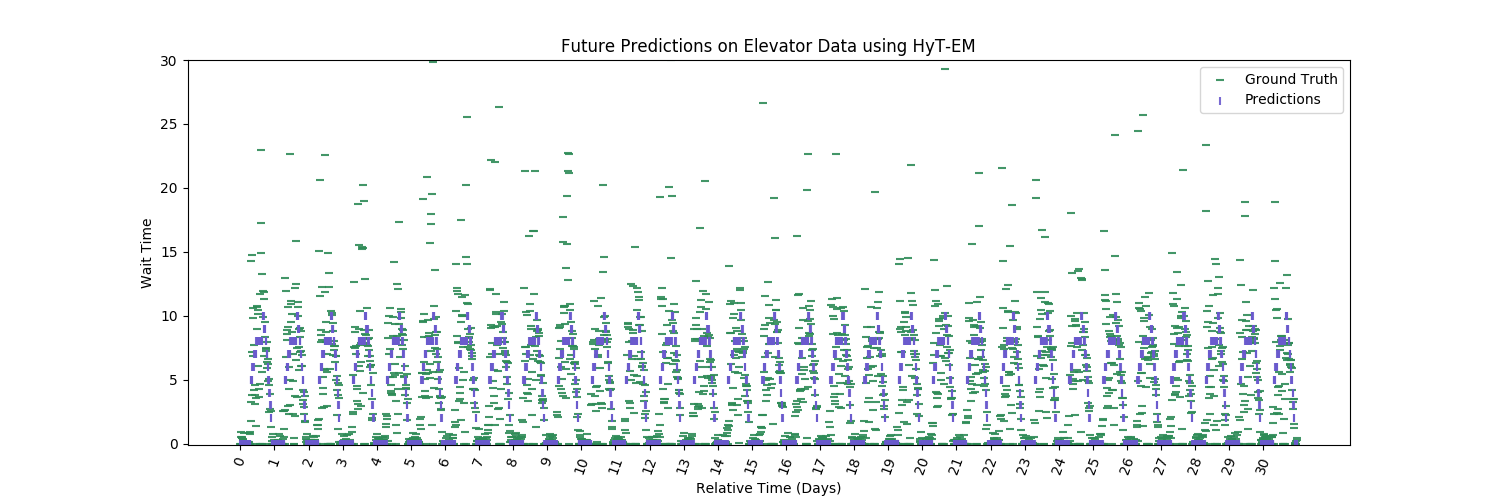
\includegraphics[width = 3in]{images/results/Future_elevator_HyT-EM.png}}
  %  \end{tabular}
  %\end{figure}


  \vspace*{-.75cm}


\begin{table}[h!]
  \centering
  \resizebox{\textwidth}{!}{%
    \begin{tabular}{|l|l|l|l|l|}
      \hline
      & DMM & Gaussian & FreMEn  & Hypertime \\ \hline
      Average Additional Wait Time (Seconds)         & 3.06    & 3.25     & 2.12    & 1.92      \\ \hline
      Computation Time (Milliseconds)                       & 610     & 60       & 70      & 7690      \\ \hline
      Memory Usage (KB)                                     & 31092   & 34636    & 34672   & 67788     \\ \hline
    \end{tabular}%
  }
  \caption{Elevator Wait Time Overview}
  \label{table:Elevator_Wait_Time_Overview}
\end{table}


  \begin{figure}
    \vspace*{-1cm}
    \hspace*{-1cm}
    {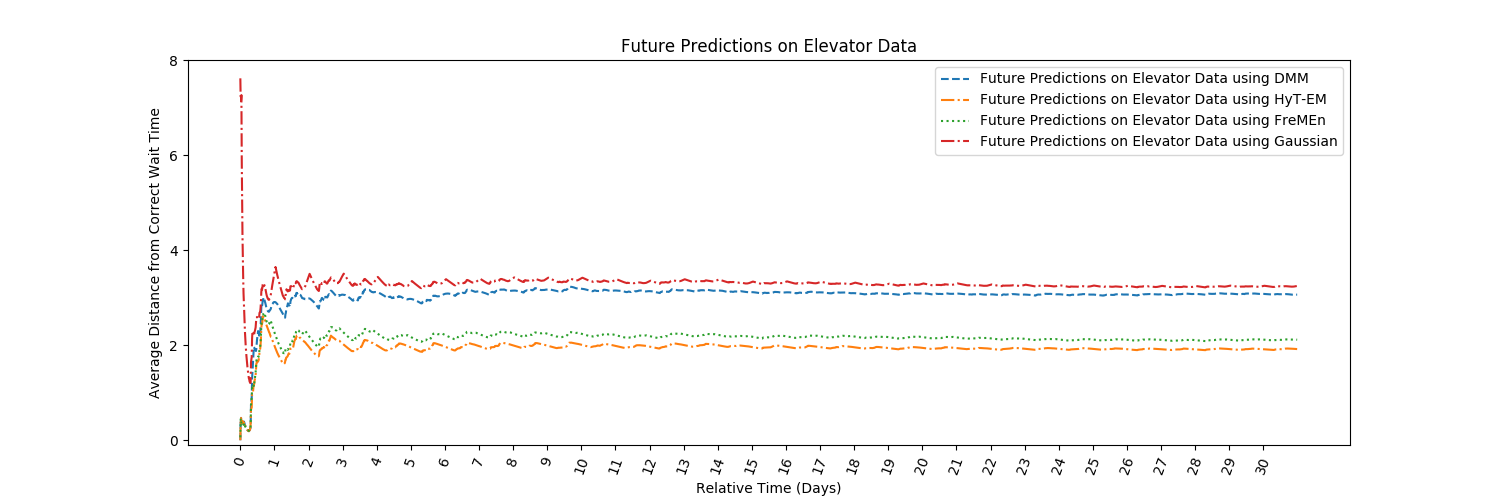
\includegraphics[width = 5in]{images/results/Future_Predictions_on_Elevator_Data.png}}
    %\caption{Layout}
  \end{figure}

\end{frame}


\begin{frame}[t]{Busy Elevator}
 \framesubtitle{Binary vs Non-Binary Predictions}

 \vspace*{-1.6cm}
 \hspace*{-1.0cm}
  \begin{figure}[!Hp]
    \begin{tabular}{cc}
      {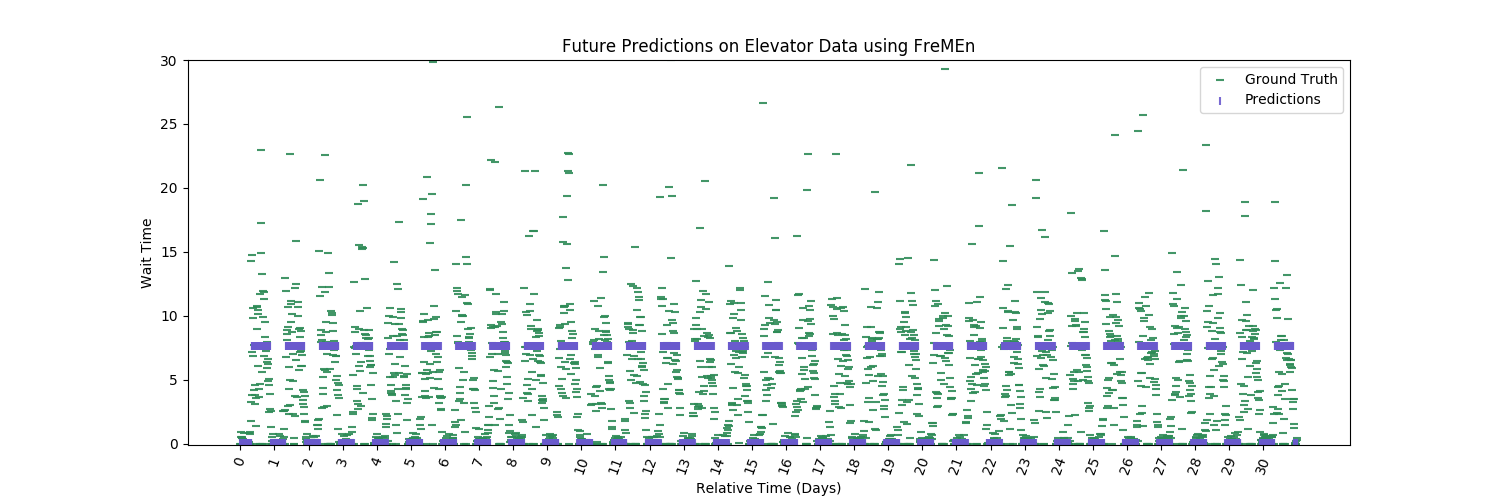
\includegraphics[width = 4.25in]{images/results/Future_elevator_FreMEn.png}} \\
      {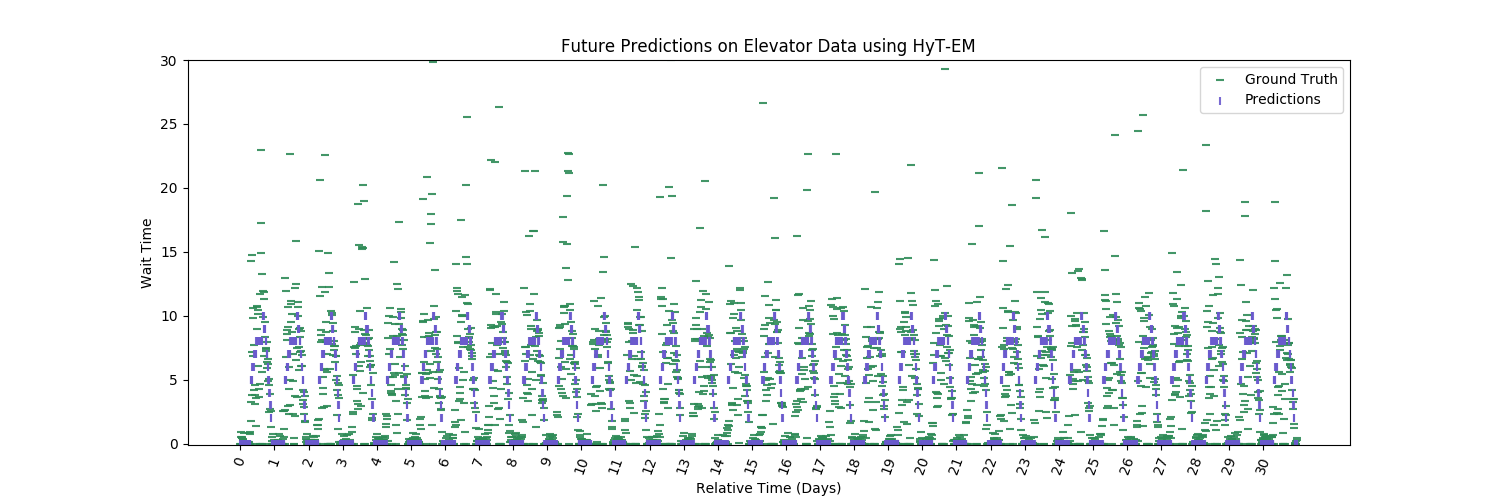
\includegraphics[width = 4.25in]{images/results/Future_elevator_HyT-EM.png}}
    \end{tabular}
  \end{figure}

\end{frame}



\begin{frame}[t]{Experiment Conclusions}
  \framesubtitle{Data Grouping Techniques}
  \vspace*{-.25cm}
  \setlength\itemsep{1.25em}

  \begin{itemize}
    \item \textbf{Black Box - General Grouping}
      \begin{itemize}
        \item Never provides invalid predictions
        \item High accuracy with large bounds
      \end{itemize}

    \item \textbf{Grey Box - Temporal Grouping}
      \begin{itemize}
        \item Decent overall performance
        \item Susceptible to invalid predictions with limited data
      \end{itemize}

    \item \textbf{White Box - Hypertime Cluster Grouping}
      \begin{itemize}
        \item Best all around performance
        \item Rarely if ever susceptible to invalid predictions
        \item Groupings limited to the number of internal clusters
      \end{itemize}

    \item \textbf{White X Grey Box - Combined Grouping}
      \begin{itemize}
        \item Requires extremely large datasets
        \item Tends towards being overly specific
        \item Performance closest to the lowest of the combined models
      \end{itemize}

  \end{itemize}
\end{frame}



\begin{frame}[t]{Experiment Conclusions}
  \framesubtitle{Confidence Estimating Techniques}
  \vspace*{+.25cm}

  \begin{itemize}
  \setlength\itemsep{1.25em}
    \item \textbf{Confidence Intervals}
      \begin{itemize}
        \item Describes general trend of behaviors
        \item Smaller bounds at the cost of accuracy
        \item Best fit for models representing discrete changes
      \end{itemize}

    \item \textbf{Two Sigma}
      \begin{itemize}
        \item Larger more accurate bounds
        \item Better encapsulation of environmental variance
      \end{itemize}

  \end{itemize}
\end{frame}


\begin{frame}[t]{Recommendations for ROPOD}
  %\framesubtitle{Hypertime with Caveats}
  %\vspace*{+.25cm}

  \begin{itemize}
  \setlength\itemsep{1.00em}
    \item \textbf{Data Grouping - White Box/Hypertime Clusters}
      \begin{itemize}
        \item Avoids issues related to small datasets
        \item Groups and generalizes underlying behaviors well
        \item Multi-model fusion of also of potential interest
      \end{itemize}

    \item \textbf{Confidence Estimates - 2$\sigma$}
      \begin{itemize}
        \item Best for generalizing dynamic range of behaviors
      \end{itemize}

    \item \textbf{Implementation}
      \begin{itemize}
        \item Collect data as often as possible
        \item Storage of spatio-temporal data on central server
        \item Docker container of quick deployment
        \item Trainings overnight every week or so
      \end{itemize}

  \end{itemize}

\end{frame}


\begin{frame}[t]{Contributions}

  \begin{itemize}
    \setlength\itemsep{1em}
        \item Presented methodology for developing confidence estimation techniques for spatio-temporal models

        \item Introduced a novel prediction method for Hypertime

        \item Provided new real-world datasets with varying noise and data density

        \item Designed and evaluated multiple confidence estimation for Hypertime

        \item Demonstrated multi-model prediction fusion

  \end{itemize}

\end{frame}


\begin{frame}[t]{Future Work}

  \begin{itemize}
    \setlength\itemsep{1em}
      \item Fusion of multiple different model types
      \item Investigation into other data grouping and confidence estimate techniques
      \item Differentiate between large bounds from lack of data and actual behaviors
      \item Leverage confidence estimates to know when and where to explore
      \item Further data visualization for increased prediction comprehension

  \end{itemize}

\end{frame}


\begin{frame}

  \centering \huge
  \emph{Thank You!} \\
  \vspace*{1cm}
  \large
  \emph{Any Questions\textbf{?}}

\end{frame}

\begin{frame}[allowframebreaks]{Bibliography}
  \begin{thebibliography}{9}
    \bibitem{Krajnik2015}
        \emph{FreMEn: Frequency Map Enhancement for Long-Term Mobile Robot Autonomy in Changing Environments}
        T. Krajník, J. Fentanes, J. Santos, \& T. Duckett,
        ICRA Workshop on Visual Place Recognition in Changing Environments
        2015
      \bibitem{Krajnik2018}
        \emph{Warped Hypertime Representations for Long-term Autonomy of Mobile Robots},
        T. Krajnik, T. Vintr, S. Molina, J.P. Fentanes, G. Cielniak, \& T. Duckett,
        2018
      \bibitem{Massey2019}
        \emph{Comparative Analysis of Techniques for Spatio-Temporal World Modeling},
        E.O. Massey, E. Prassler, A.O. S{\'{a}}inz, \& S. Blumenthal,
        2019
      \bibitem{Confidence2019}
        \emph{Oxford University Press (OUP)},
        Lexico.com,
        2019
      \bibitem{Geifman2018}
        \emph{Bias-Reduced Uncertainty Estimation for Deep Neural Classifiers},
        Y. Geifman, G. Uziel, R. El-Yaniv,
        2018
      \bibitem{Shrestha2006}
        \emph{Machine learning approaches for estimation of prediction interval for the model output},
        D.L. Shrestha, D.P. Solomatine,
        2006

  \end{thebibliography}
\end{frame}




\end{document}
